\chapter{The Wireless Channel}
\label{ch:channels}
\providecommand{\chElevenFigH}[3][0.92]{\begin{figure}[H]\centering\includegraphics[width=#1\linewidth]{figs/#2}\caption{#3}\label{fig:#2}\end{figure}}

\begin{chapterintro}
Hold your phone at arm's length and look at the signal bars. Now take one step. The bars may
not change, but the signal inside the phone just rose and fell by a factor of a hundred,
several times, while you moved. It was spread over the sky by the base-station antenna,
reflected off the building across the street, bent over a rooftop, filtered through your
coat, and split into dozens of echoes that arrived at slightly different times and slightly
different frequencies, adding up here and cancelling there. Your phone sorted the mess out
without you noticing. This chapter is about the mess, and about how engineers learned to
predict it well enough to design networks that cover continents.

\end{chapterintro}

%======================================================================
\section{What the channel does to a signal}
\label{sec:ch11:overview}
%======================================================================

A cellular base station pushes something like 40 watts into each of its antennas. A phone at the
edge of the cell, a kilometre or two away, works happily with a few femtowatts. Put those two
numbers on one ruler (Figure~\ref{fig:ch11_power_ladder}) and the gap is staggering: roughly
175\,dB, a factor of more than $10^{17}$. Almost all of it is lost in the air between them, and
the phone still decodes megabits per second. Understanding where that power goes, and why it
arrives in such a jittery state, is the job of this chapter.

\begin{figure}[H]\centering
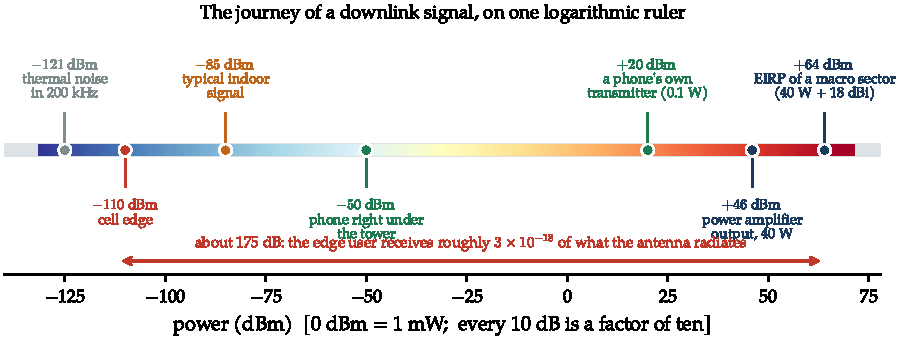
\includegraphics[width=0.86\linewidth]{figs/ch11_power_ladder}
\caption{The journey of a downlink signal on one logarithmic ruler. A macro-cell
sector radiates around $+64$\,dBm of EIRP; a phone at the cell edge works with about $-110$\,dBm, only
some 10\,dB above the thermal noise in a narrowband channel. Decibels are the only sane way to
keep score over 175\,dB.}\label{fig:ch11_power_ladder}
\end{figure}

A radio link is a transmitter, a receiver, and everything in between. That ``everything'' is the
reason wireless communication is a distinct discipline from wireline. A copper pair or an optical
fibre is a stable, well-characterised filter: you measure it once and design to it. The wireless
channel changes when the user moves a few centimetres, when a bus drives past, when it rains,
when the Sun rises over the ionosphere. It is also shared: every transmitter in the band is part
of every receiver's channel.

\mdcphoto[0.36]{ch11_cell_tower}{The top of a cellular monopole, with several tiers of antennas.
Each tall white panel is a sector antenna, a vertical column of radiating elements that squeezes
the beam into a thin horizontal slice and points it a few degrees below the horizon; three or
more panels around the pole cover the full circle. Everything this chapter says about
gain, beamwidth, downtilt and polarization is visible in this one photograph.}

Engineers tame the complexity by separating effects that happen on different scales of distance
and time. Figure~\ref{fig:ch11_scales} shows a simulated drive away from a 2\,GHz base station,
and in it three distinct behaviours are visible.

\begin{enumerate}
\item \textbf{Path loss.} The mean received power falls steadily with distance---in free space
as $d^{-2}$, in a city more like $d^{-3.5}$. This is the \emph{large-scale} trend, varying over
hundreds of metres to kilometres. It sets the size of a cell.
\item \textbf{Shadowing.} Around that trend the local mean wanders by several decibels as the
receiver passes behind buildings, hills and trees. The fluctuation is correlated over tens of
metres and, measured in decibels, is well described by a Gaussian distribution---hence the
name \emph{log-normal shadowing}. It sets the \emph{margin} a cell must be designed with.
\item \textbf{Small-scale (multipath) fading.} Superimposed on both are rapid fluctuations of
20--40\,dB over distances of a fraction of a wavelength---7.5\,cm at 2\,GHz. These are caused by
the interference of many echoes, and they are what makes the mobile channel hard: they set the
error-rate behaviour of the modem, the design of its equalizer, its pilots and its codes.
\end{enumerate}

\mdcfig{ch11_scales}{The three scales of propagation, simulated at 2\,GHz. (a) Path loss (red)
falls smoothly with distance; log-normal shadowing (navy, $\sigma=7$\,dB, correlated over
about 50\,m) wanders around it; multipath fading (grey) adds rapid excursions of tens of
decibels. (b) A 2\,m stretch at 400\,m: the local mean barely changes, but the received
power drops by 20--35\,dB at nulls spaced roughly half a wavelength apart.}

\begin{analogy}[A drive through hill country]
Think of the received power as the altitude of a road you are driving. \emph{Path loss} is the
long, steady descent from the mountains to the sea: you can see it on a map. \emph{Shadowing} is
the rolling hills along the way, each a few hundred metres long, that a map-maker would smooth
over. \emph{Multipath fading} is the gravel and potholes: invisible on any map, changing every
few centimetres, and the thing that actually rattles your teeth. The limit of the analogy: real
potholes stay put, while multipath nulls move every time anything in the scene moves.
\end{analogy}

Mathematically, all three effects live inside one object. The received complex baseband
signal is
\begin{equation}
y(t)=\int h(\tau,t)\,x(t-\tau)\,d\tau+n(t),
\label{eq:ch11:ltv}
\end{equation}
a \emph{linear time-varying} filter $h(\tau,t)$---the response at time $t$ to an impulse sent
$\tau$ seconds earlier---plus the noise of Chapter~\ref{ch:noise}. In words: the channel is an
echo machine whose echoes keep changing. Path loss and shadowing fix the average energy of $h$;
multipath fixes its structure in delay $\tau$; motion makes it change with $t$. The chapter
works outward from the simplest case (one path in empty space) to the full statistical
description of $h(\tau,t)$ in Section~\ref{sec:ch11:wssus}, and then to the models that
standards bodies use to test real equipment.

\begin{keyidea}[Three scales, three design problems]
Path loss decides \emph{whether} a link can close and how big a cell can be; it is handled by
the link budget, antenna gain and transmit power. Shadowing decides \emph{how reliably} it
closes across a coverage area; it is handled by margin, cell overlap and handover.
Multipath fading decides \emph{how the modem must be built}; it is handled by equalization,
OFDM, diversity, interleaving and coding. Keep the three separate in your head and most
wireless design questions sort themselves into the right box.
\end{keyidea}

Everything in the first ten chapters assumed a kind channel: a wire, a filter, a little white
noise. The radio channel is not kind. The rest of this chapter builds its engineering model from
the ground up: from Maxwell's equations to the antenna, from the Friis equation to a complete
link budget, from reflection and diffraction to the ionosphere and the rain cell, from Okumura's
Tokyo drive tests to the 3GPP models used to design 5G, and from the physics of multipath to the
statistics---Rayleigh, Rice, Clarke, Bello---that every modem designer lives by. We finish by
showing how the channel writes the numbers inside the standards: why LTE subcarriers are
15\,kHz apart, why the cyclic prefix is 4.7\,$\mu$s, and why no serious wireless system works
without diversity.

%======================================================================
\section{From Maxwell to the antenna}
\label{sec:ch11:maxwell}
%======================================================================

In 1865 a Scottish physicist sat down with four equations and two numbers measured on a lab bench
with capacitors and coils, and out fell the speed of light. Nobody had told James Clerk Maxwell
that light was electrical. The mathematics did.

Radio waves are solutions of Maxwell's equations. Change an electric field and you create a
magnetic one; change the magnetic field and you create an electric one; the pair can chase each
other through empty space forever, each regenerating the other, at a speed fixed by two constants
of nature (Figure~\ref{fig:ch11_wave_eh}). That is all a radio wave is.

\mdcside[0.4]{ch11_wave_eh}{A plane wave far from its antenna: the electric field (red) and
magnetic field (navy) are perpendicular to each other and to the direction of travel, and rise
and fall together.}

In a source-free, linear, homogeneous medium with permittivity $\epsilon$ and permeability
$\mu$, Maxwell's equations combine into a wave equation whose solutions travel at
$c=1/\sqrt{\mu\epsilon}$. In vacuum this is $299\,792\,458$\,m/s. Maxwell computed it in 1865
from the measured electric and magnetic constants, noticed that it equalled the speed of light,
and concluded that light was an electromagnetic wave. Radio is the same wave at a lower
frequency; the wavelength $\lambda=c/f$ is 300\,m at 1\,MHz, 1\,m at 300\,MHz, 10\,cm at 3\,GHz
and 1\,cm at 30\,GHz. Keep those four numbers in your pocket: almost every antenna and
propagation effect in this chapter scales with the wavelength, and the wavelength tells you at a
glance whether a building, a raindrop or a person is ``large'' or ``small'' to the wave.

Waves are launched by accelerating charge. Far enough from any antenna the field becomes, locally,
a \emph{plane wave}: $\vect{E}$ and $\vect{H}$ perpendicular to each other and to the direction of
travel, in phase, with a fixed ratio $|\vect{E}|/|\vect{H}|=\eta_0\approx377\,\Omega$, the
\emph{impedance of free space}. The power flowing through each square metre is the Poynting
vector $S=|\vect{E}|^2/\eta_0$ (RMS field), in W/m$^2$.



That is almost all the electromagnetics a communication engineer needs day to day, plus one
geometric fact: in the far field of \emph{any} antenna, energy conservation forces the power
density to fall as $1/r^2$, because the same power crosses spheres of area $4\pi r^2$. The
amplitude falls as $1/r$, which is why field strength in broadcasting is quoted in dB$\mu$V/m
and falls 20\,dB per decade of distance in free space. Everything else---the antenna's pattern,
reflection, diffraction, absorption---modifies this spherical spreading.

\begin{analogy}[Paint from a spray can]
Point a spray can at a wall one metre away and you get a small, dense patch of paint. Step back
to two metres and the same paint covers four times the area, so the coat is a quarter as thick;
at three metres it is a ninth (Figure~\ref{fig:ch11_spray}). No paint was lost: it was spread
thinner. Free-space ``path loss'' is exactly this. The limits: real paint does not interfere
with itself, and a radio wave's ``coat'' is measured with an antenna of a certain catching area,
which, as we shall see, is where frequency sneaks into the story.
\end{analogy}

\chElevenFigH[0.5]{ch11_spray}{The spray-can picture of free-space loss: the same number of dots
spread over arcs at $d$, $2d$ and $3d$. The area grows as $d^2$, so the density falls as $1/d^2$.}

\begin{deeper}[From Maxwell's equations to the far field]
In a source-free, linear, homogeneous medium the equations are
\begin{equation}
\nabla\times\vect{E}=-\mu\frac{\partial\vect{H}}{\partial t},\qquad
\nabla\times\vect{H}=\epsilon\frac{\partial\vect{E}}{\partial t},\qquad
\nabla\cdot\vect{E}=0,\qquad\nabla\cdot\vect{H}=0 .
\end{equation}
Take the curl of the first and substitute the second to get the wave equation
$\nabla^2\vect{E}=\mu\epsilon\,\partial^2\vect{E}/\partial t^2$, whose solutions travel at
$c=1/\sqrt{\mu\epsilon}$.

The simplest radiator, a short current element of length $\ell\ll\lambda$ carrying current $I$,
produces fields with three kinds of term: one falling as $1/r^3$ (the quasi-static dipole field),
one as $1/r^2$ (the induction field) and one as $1/r$. Only the last carries power to infinity.
At distances beyond about $\lambda/2\pi$ the $1/r$ term dominates, and far enough away---beyond
the \term{Fraunhofer distance} $2D^2/\lambda$ for an antenna of largest dimension $D$---the
field is locally a plane wave with $|\vect{E}|/|\vect{H}|=\eta_0=\sqrt{\mu_0/\epsilon_0}
\approx377\,\Omega$.
\end{deeper}

\begin{history}[Maxwell, Hertz and the first antenna]
James Clerk Maxwell published ``A Dynamical Theory of the Electromagnetic Field'' in 1865,
predicting electromagnetic waves that nobody had seen. Heinrich Hertz generated and detected
them in Karlsruhe between 1886 and 1888, using a spark gap across a pair of rods---a
dipole---as the transmitter and a small loop with a microscopic gap as the receiver
(Figure~\ref{fig:ch11_hertz}). He worked with wavelengths from tens of centimetres to several
metres (frequencies of tens to hundreds of megahertz), demonstrated reflection from a zinc
sheet, focusing by a parabolic reflector, refraction through a prism of pitch and polarisation
by a wire grid. In other words, Hertz's laboratory already contained the dipole, the dish and
the polariser of this chapter. He reportedly saw no practical use for his waves; within a decade
Marconi, Popov and others were sending messages with them.
\end{history}

\mdcphoto[0.6]{ch11_hertz}{Apparatus for repeating Hertz's experiments, from a 1912 catalogue of teaching equipment: a spark transmitter driven by an induction coil (left) and a receiver (right), each placed at the focus of a metal reflector that beams the waves, just as Hertz focused his with a parabolic mirror. Every dish antenna since is a descendant.}

%======================================================================
\section{Antennas for communication engineers}
\label{sec:ch11:antennas}
%======================================================================

Walk down any city street and count the antennas. The white panels on the rooftop, the stubby
whip on a delivery van, the grey dish on a balcony, the flat square on a camper van roof, the
invisible strips of copper inside the phone in your pocket. They look nothing alike, yet a
communication engineer describes every one of them with the same half-dozen numbers, because
those numbers drop straight into the link budget.

An antenna is a transducer between a guided wave on a transmission line and a free wave in
space. A communication engineer rarely designs one, but must be fluent in its vocabulary.

\subsection{Pattern, directivity and gain}

The \term{radiation pattern} $U(\theta,\phi)$ is the power radiated per unit solid angle in
each direction. An \emph{isotropic} antenna---a mathematical fiction that radiates equally
in all directions---would produce $U_0=P_{\text{rad}}/4\pi$. The \term{directivity} is the ratio
of the maximum radiation intensity to this isotropic average,
\begin{equation}
D=\frac{U_{\max}}{P_{\text{rad}}/4\pi}=\frac{4\pi}{\Omega_A},
\qquad
\Omega_A=\iint\frac{U(\theta,\phi)}{U_{\max}}\,d\Omega ,
\end{equation}
where $\Omega_A$ is the \emph{beam solid angle}: the solid angle into which all the power would
go if the intensity were uniform at its peak value. A narrow beam means a small $\Omega_A$ and
a large directivity. For a pencil beam with half-power beamwidths $\theta_E$ and $\theta_H$
in degrees in the two principal planes, a useful approximation is
$D\approx 41\,253/(\theta_E\theta_H)$ (the number is the solid angle of a sphere, $4\pi$
steradians, in square degrees); practical antennas with sidelobes achieve closer to
$30\,000/(\theta_E\theta_H)$.

\mdcfig{ch11_pattern3d}{Gain is concentration, not creation. (a) A half-wave dipole radiates a
doughnut, strongest broadside to the wire and zero along it. (b) An $8\times4$ panel of patch
elements squeezes almost all its power into one forward beam, with a few weak sidelobes (plotted on
a 30\,dB logarithmic scale so the sidelobes are visible).}

\term{Gain} includes losses: $G=e_{\text{rad}}D$, where the radiation efficiency $e_{\text{rad}}$
accounts for ohmic loss in conductors and dielectrics. Gain is what the link budget uses,
expressed in dBi (decibels relative to isotropic). A second reference, the half-wave dipole,
gives dBd; since a dipole has 2.15\,dBi, $G_{\text{dBi}}=G_{\text{dBd}}+2.15$. Antenna gain
does not create power---an antenna is passive---it redistributes it: what one direction
gains, others lose (Figure~\ref{fig:ch11_pattern3d}).

\begin{analogy}[A bare bulb and a flashlight]
A 5\,W bare bulb lights a whole room dimly; put the same bulb in a flashlight with a mirror and
it throws a bright spot across the garden, while the rest of the garden goes dark. The mirror
added no watts. ``Gain'' is the brightness of the spot compared with the bare bulb. The
analogy's limit: a flashlight's mirror is many wavelengths of light across, while many radio
antennas are only a fraction of a wavelength, which is why small antennas cannot have narrow
beams.
\end{analogy}

\subsection{Effective aperture}

A receiving antenna presents an \term{effective aperture} $A_e$: the area which, multiplied by
the incident power density, gives the power delivered to a matched load. Think of it as the size
of the bucket the antenna holds out in the rain of radio energy. The fundamental relation between
the transmitting property (gain) and the receiving property (aperture) is
\begin{equation}
A_e=\frac{\lambda^2}{4\pi}\,G .
\label{eq:ch11:aperture}
\end{equation}
Read it in words: for a given gain, the bucket shrinks with the square of the wavelength. An
antenna that is equally ``directive'' at 900\,MHz and at 28\,GHz catches a thousand times less
power at the higher frequency, simply because it is a thousand times smaller in area.

\begin{deeper}[Why $A_e/G=\lambda^2/4\pi$ for every antenna]
The relation follows from reciprocity together with a thermodynamic argument: an antenna in a
black-body enclosure at temperature $T$, connected to a resistor at the same temperature, must
absorb from the radiation exactly as much power ($kTB$) as the resistor sends out through the
antenna; otherwise heat would flow between two bodies at the same temperature, violating the
second law. Working that through for any antenna gives $A_e/G=\lambda^2/4\pi$, the effective
aperture of an isotropic antenna. No antenna can beat it, and no clever design can make it
depend on anything except the wavelength.
\end{deeper}

For physical apertures---horns, dishes, flat panels---the effective aperture is a fraction $\eta$
(the \emph{aperture efficiency}, typically 0.5--0.75 for dishes) of the physical area, so a dish of
diameter $D$ has
\begin{equation}
G=\eta\left(\frac{\pi D}{\lambda}\right)^2,\qquad
\theta_{3\,\mathrm{dB}}\approx 70\,\frac{\lambda}{D}\ \text{degrees}.
\label{eq:ch11:dish}
\end{equation}
Gain grows with the square of the diameter measured in wavelengths, and the beamwidth shrinks in
proportion to $\lambda/D$ (Figure~\ref{fig:ch11_antennas}c). Double the dish and you gain 6\,dB
and halve the beam; double the frequency with the same dish and you get the same.

\chElevenFigH[0.5]{ch11_dish_beam}{The worked example as patterns: the same 60\,cm dish (uniform
circular aperture) at 12\,GHz and at 1.2\,GHz. At 12\,GHz the main lobe is a few degrees wide; at
1.2\,GHz it swallows the whole neighbourhood of the geostationary arc.}

\begin{worked}[A satellite TV dish]
A 60\,cm offset dish receives Ku-band broadcast at 12\,GHz ($\lambda=2.5$\,cm) with aperture
efficiency 0.65. Its gain is $0.65\,(\pi\times0.6/0.025)^2=0.65\times5685\approx3700$, or
35.7\,dBi, and its beamwidth is about $70\times0.025/0.6\approx2.9^\circ$. That is narrow enough
to discriminate between geostationary satellites spaced $2^\circ$ apart only with the help of
the sidelobe envelope, which is why regulators constrain both satellite spacing and small-dish
patterns. The same dish at 1.2\,GHz would have 20\,dB less gain and a $29^\circ$ beam: useless
for picking one satellite out of the arc (Figure~\ref{fig:ch11_dish_beam}).
\end{worked}



\mdcphoto[0.7]{ch11_dsn}{The 70\,m antenna of NASA's Deep Space Network at Goldstone, California.
At X band (8.4\,GHz) a dish this size has a gain of roughly 74\,dBi and a beam about
$0.04^\circ$ wide---the reason a spacecraft transmitter of a few tens of watts can be heard from
beyond Pluto (Figure~\ref{fig:ch11_antennas}c plots the gain of this dish against frequency).}

\subsection{Polarization}

The direction of the electric field defines the \term{polarization}
(Figure~\ref{fig:ch11_polarization}). A vertical dipole radiates vertical linear polarization; two
orthogonal dipoles driven $90^\circ$ apart radiate circular polarization, in which the field vector
rotates once per cycle like a corkscrew. If the receive antenna's polarization is not matched to the
incoming wave, only the projection is received: the \emph{polarization loss factor} for linear
polarizations at angle $\psi$ is $\cos^2\psi$---3\,dB at $45^\circ$ and, in theory, infinite at
$90^\circ$ (in practice 20--30\,dB, limited by imperfections and depolarising scatter).
Linear-to-circular always costs 3\,dB.

\mdcfig{ch11_polarization}{Three polarizations, drawn as the tip of the electric-field vector
along the direction of travel. (a) Vertical linear: the field swings up and down. (b) Slant
$45^\circ$: the trick used by cellular panels, which carry a $+45^\circ$ and a $-45^\circ$ antenna
in one housing. (c) Circular: the field rotates like a corkscrew; GPS and most low-frequency
satellite links use it.}

Engineers exploit polarization in three ways. First, orthogonal polarizations are two nearly
independent channels: satellite systems reuse every frequency twice on H and V (or left- and
right-hand circular), and microwave backhaul links carry two data streams on one frequency
with cross-polarization interference cancellation. Second, circular polarization is immune to
the Faraday rotation that the ionosphere imposes on linearly polarized waves, which is why GPS
and most satellite links below 10\,GHz use it. Third, cellular base stations use
\emph{$\pm45^\circ$ cross-polarized} antennas: in a cluttered environment the two polarizations
fade nearly independently, giving diversity (Section~\ref{sec:ch11:ber}) without a second
antenna location.

\subsection{EIRP and ERP}

Regulators care about what leaves the antenna in its strongest direction. The
\term{effective isotropic radiated power} is
\begin{equation}
\mathrm{EIRP}=P_tG_t\quad\text{(in dB: }P_t\,[\mathrm{dBm}]+G_t\,[\mathrm{dBi}]-L_{\text{feed}}\text{)},
\end{equation}
the power an isotropic radiator would need to produce the same peak power density. Broadcast
and land-mobile rules often use the \emph{effective radiated power} ERP relative to a dipole,
so $\mathrm{ERP}=\mathrm{EIRP}-2.15$\,dB. Wi-Fi limits, satellite footprints and cellular licences
are all written in EIRP or ERP, not in transmitter power, which is why a higher-gain antenna
usually requires a lower transmitter power. In the flashlight picture: the regulator limits the
brightness of the spot, not the wattage of the bulb.

\subsection{A field guide to antennas}

Antennas come in a zoo of shapes, but six species cover most of what a communication engineer
meets. Here they are, from the humble wire to the electronically steered panel.

\begin{description}[style=unboxed,leftmargin=0pt]
\item[The half-wave dipole.] Two quarter-wave arms fed in the centre: 2.15\,dBi gain, a doughnut
pattern with nulls along the axis (Figure~\ref{fig:ch11_antennas}a), input resistance about
73\,$\Omega$. A \emph{monopole} over a ground plane is half a dipole, with 36\,$\Omega$ and
twice the peak gain in its half-space. Broadcast towers, car roofs and handheld radios use it.
\item[The Yagi--Uda array.] A driven dipole with a reflector behind and several directors in
front, invented in Japan in 1926; 7--15\,dBi, the rooftop TV antenna
(Figure~\ref{fig:ch11_yagi}).
\item[The patch.] A rectangle of metal about $\lambda/2$ long over a ground plane on a circuit
board: cheap, flat, 6--9\,dBi, narrow bandwidth. It is the building block of GPS antennas,
Wi-Fi access points and phased arrays.
\item[The horn.] A flared waveguide: 10--25\,dBi, very wide bandwidth, precisely calculable
gain. Horns feed dishes and serve as gain standards in measurements.
\item[The parabolic dish.] A reflector that turns a spherical wave from its focus into a plane
wave: 30--75\,dBi. Satellite ground stations, microwave backhaul and deep space.
\item[The phased array.] $N$ elements whose signals are combined with controlled phases. The
pattern is the element pattern times the \emph{array factor}; for a uniform linear array with
spacing $d$ and progressive phase shift chosen to steer to angle $\theta_0$,
\begin{equation}
\mathrm{AF}(\theta)=\frac{\sin(N\psi/2)}{N\sin(\psi/2)},\qquad
\psi=\frac{2\pi d}{\lambda}(\sin\theta-\sin\theta_0).
\end{equation}
The peak gain grows as $N$ (10\,dB for 10 elements); the beam can be moved electronically in
microseconds; and spacing must be at most $\lambda/2$ to avoid \emph{grating lobes}---copies
of the main beam in unwanted directions (Figure~\ref{fig:ch11_antennas}b). Phased arrays are
the heart of 5G millimetre-wave handsets and base stations, of Starlink user terminals
(Figure~\ref{fig:ch11_starlink}) and of modern radar. Chapter~\ref{ch:mimo} develops them fully.
\end{description}

\mdcfig{ch11_antennas}{(a) Elevation pattern of a short (Hertzian) dipole and a half-wave
dipole: both radiate a doughnut with nulls along the wire; the half-wave dipole's beam is
slightly narrower (2.15\,dBi versus 1.76\,dBi). (b) Array factor of an 8-element,
half-wavelength-spaced linear array, at broadside and steered electronically to $30^\circ$;
the beam broadens when steered. (c) Gain of a parabolic dish with 60\% efficiency versus
frequency for three diameters: a 60\,cm satellite TV dish, Voyager's 3.7\,m antenna and a
70\,m Deep Space Network dish.}



\begin{figure}[H]\centering
\begin{minipage}[t]{0.48\linewidth}\centering
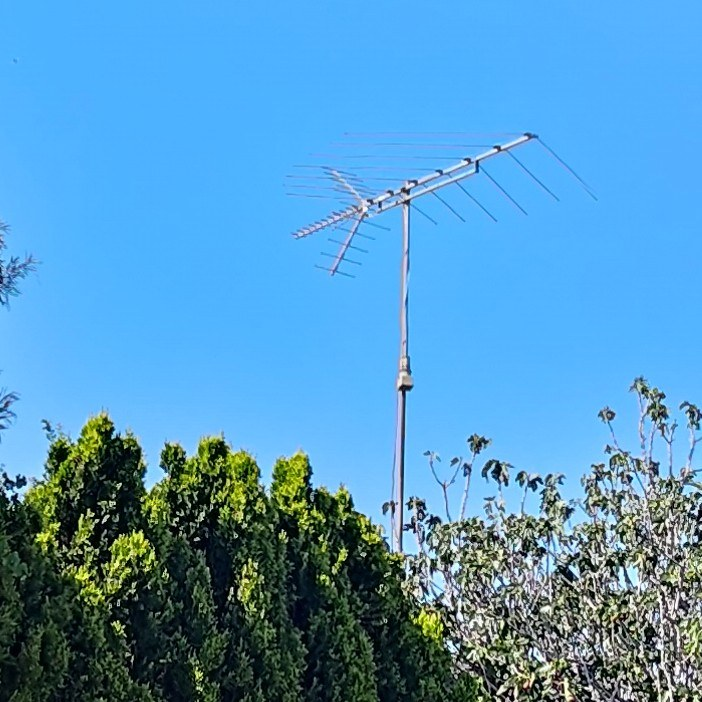
\includegraphics[width=\linewidth,height=5.2cm,keepaspectratio]{figs/photos/ch11_yagi}
\caption{A Yagi--Uda TV antenna on a rotator. The longest element at the back is the reflector; the
row of shorter rods in front are directors that pull the beam forward.\mdccredit{ch11_yagi}}
\label{fig:ch11_yagi}\end{minipage}\hfill
\begin{minipage}[t]{0.48\linewidth}\centering
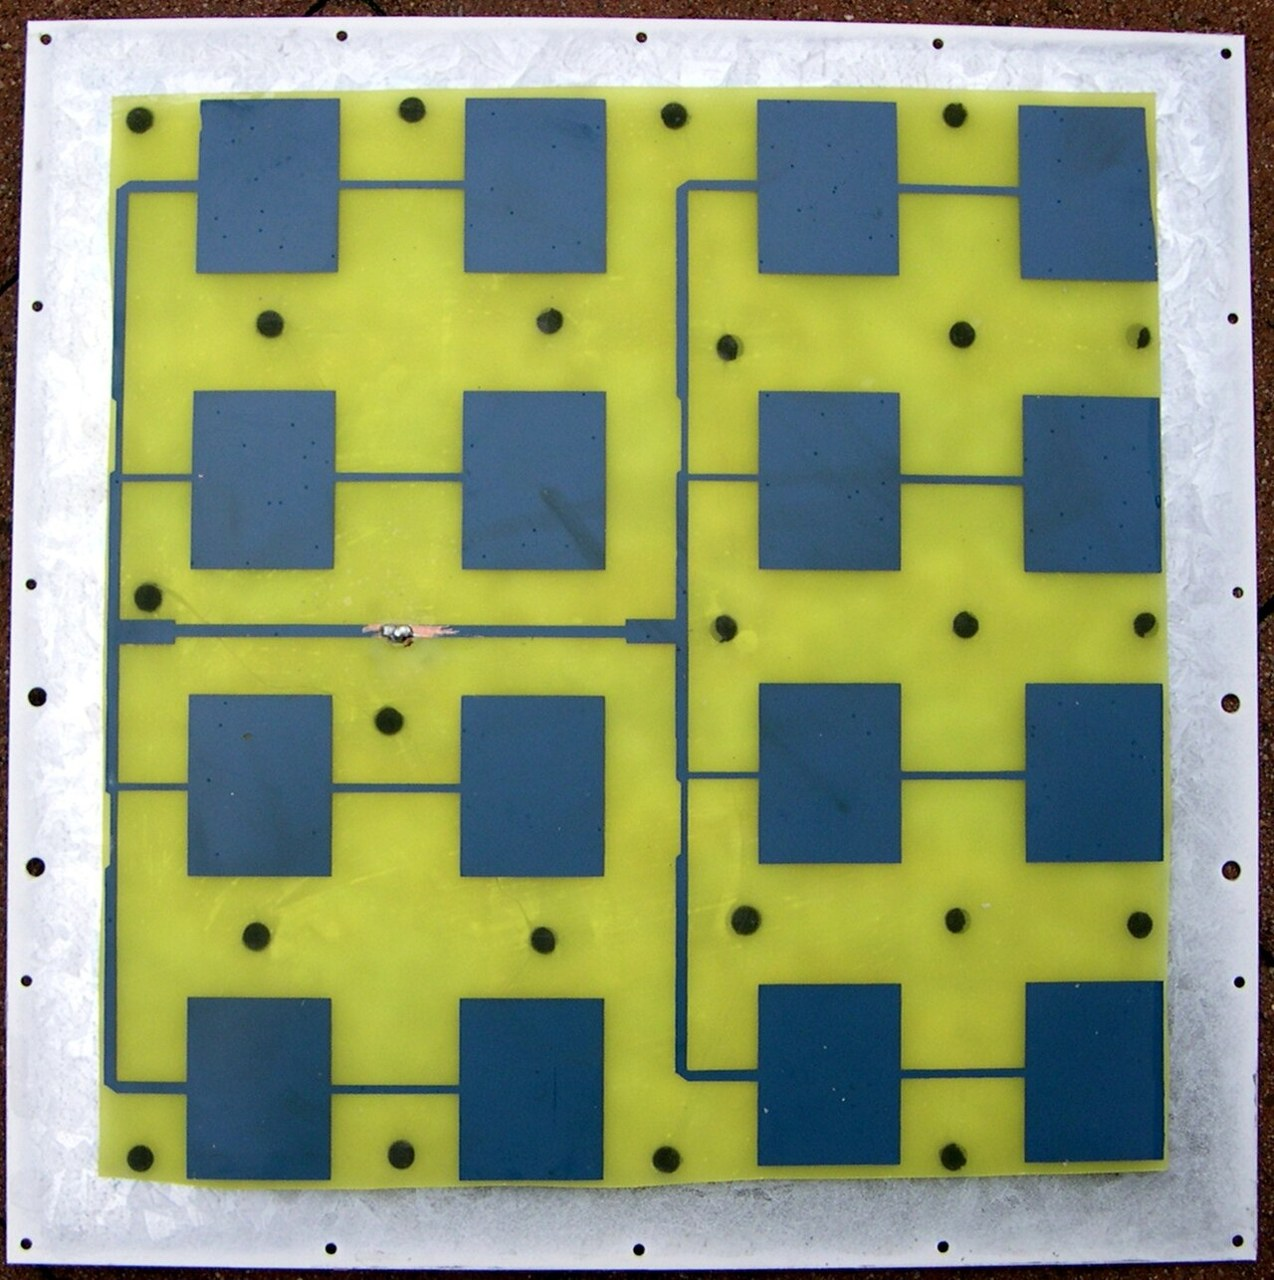
\includegraphics[width=\linewidth,height=5.2cm,keepaspectratio]{figs/photos/ch11_patch}
\caption{A flat 2.4\,GHz antenna made of sixteen patches, each a metal rectangle about half a
wavelength long over a ground plane, joined by a printed feed network. Arrays like this form most
modern panels.\mdccredit{ch11_patch}}
\label{fig:ch11_patch}\end{minipage}
\end{figure}

\begin{history}[Yagi, Uda and the antenna the world borrowed]
Shintaro Uda, working with Hidetsugu Yagi at Tohoku Imperial University in Sendai, developed the
director-array antenna in 1926; Yagi's English-language paper of 1928 brought it to the world,
which is why it often carries only his name. The design was taken up enthusiastically by radar
engineers abroad in the 1930s and 1940s. A frequently told story holds that Japanese officers,
examining captured British radar documents during the Second World War, were puzzled by
references to a ``Yagi'' antenna---not realising it was a Japanese invention. Whether or not every
detail is accurate, the antenna itself is still on millions of rooftops.
\end{history}

\mdcphoto[0.62]{ch11_horn}{The Holmdel horn antenna at Bell Labs, New Jersey, built in 1959 for
experiments with the Echo balloon satellite. Its low sidelobes made it an exceptionally quiet
receiver: in 1964--65 Arno Penzias and Robert Wilson, unable to get rid of a faint excess noise of a
few kelvin, found they were hearing the cosmic microwave background, the afterglow of the Big Bang
(Nobel Prize, 1978).}

\mdcphoto[0.6]{ch11_starlink}{A Starlink flat-panel terminal on a truck roof. Behind the plain
cover is a phased array of many small elements; the beam is steered electronically to follow
satellites racing across the sky, with no moving parts.}

\begin{inpractice}[The cellular sector antenna and the handset antenna]
A typical macro-cell site has three sectors, each served by a panel about 1.3--2\,m tall
containing a vertical column of cross-polarized patch or dipole elements
(Figure~\ref{fig:ch11_cell_tower}). The column gives a
narrow elevation beam (about $6$--$8^\circ$), the element width a horizontal half-power
beamwidth of about $65^\circ$, and the combination a gain of roughly 15--18\,dBi. The beam is
tilted a few degrees below the horizon---mechanically or, more usually now, by a remotely
adjustable electrical downtilt---to put the strongest signal inside the cell and less into
neighbours; tilt is one of the most powerful optimisation knobs an operator has. The handset
is the opposite extreme: several antennas squeezed into the edges of a metal frame, each
serving several bands, with total efficiencies often 3--6\,dB below ideal in free space and
worse when held against a head or in a hand. Link budgets therefore carry a \emph{body loss}
term of a few decibels, and 3GPP specifies over-the-air performance (total radiated power and
total isotropic sensitivity) rather than conducted numbers for many device tests.
\end{inpractice}

%======================================================================
\section{Free space and the Friis equation}
\label{sec:ch11:friis}
%======================================================================

In 1946 Harald Friis at Bell Labs wrote a short paper with a modest aim: to give radio engineers
a simple formula for the power received between two antennas in free space. It became the most
used equation in wireless engineering. Every satellite link, every Wi-Fi plan and every 5G cell
begins with it.

\subsection{Derivation}

The derivation is the spray can of the previous section, plus a bucket. Put an isotropic
transmitter radiating $P_t$ at the centre of a sphere of radius $d$. The power density on the
sphere is $P_t/4\pi d^2$. A transmit antenna of gain $G_t$ multiplies it by $G_t$ in the direction
of its peak, and a receive antenna of effective aperture $A_r$ collects
\begin{equation}
P_r=\frac{P_tG_t}{4\pi d^2}\,A_r=P_tG_tG_r\left(\frac{\lambda}{4\pi d}\right)^2,
\label{eq:ch11:friis}
\end{equation}
where the second form used Equation~\eqref{eq:ch11:aperture}. This is the Friis transmission
equation, already met as Equation~\eqref{eq:ch03:friistx}. The factor $(4\pi d/\lambda)^2$ is the
\term{free-space path loss}; in engineering units,
\begin{equation}
L_{\text{fs}}\,[\mathrm{dB}]=32.45+20\log_{10}f_{\mathrm{MHz}}+20\log_{10}d_{\mathrm{km}}
=92.45+20\log_{10}f_{\mathrm{GHz}}+20\log_{10}d_{\mathrm{km}} .
\label{eq:ch11:fspl}
\end{equation}
At 2\,GHz and 1\,km it is 98.5\,dB; at 28\,GHz, 121.4\,dB. Every doubling of distance
costs 6\,dB; every decade, 20\,dB (Figure~\ref{fig:ch11_fspl_lines}).

\chElevenFigH[0.5]{ch11_fspl_lines}{Free-space loss between isotropic antennas: straight lines on a log
axis, 20\,dB per decade of distance, shifted down by 20\,dB per decade of frequency.}

 The equation is valid in the far field of both antennas, with
matched polarizations and impedances and nothing in the way---conditions that point-to-point
microwave and satellite links approach, and that a phone in a street almost never does.

\begin{tryit}[Lab 22: the Friis calculator]
Open \lab{lab22\_propagation\_link\_budget.py} and choose the free-space model. Drag the distance
slider from 100\,m to 10\,km and watch the received power fall exactly 20\,dB. Now hold the
distance and drag the frequency from 900\,MHz to 28\,GHz: with fixed-gain antennas you lose about
30\,dB. Finally switch both antennas to ``fixed aperture'' and repeat---the loss turns into a gain.
\end{tryit}

\subsection{Does path loss really grow with frequency?}

The frequency term in Equation~\eqref{eq:ch11:fspl} is the source of one of the most
persistent misconceptions in radio: ``high frequencies do not travel as far.'' In free space,
the wave does not know its frequency; the power density at distance $d$ is $P_tG_t/4\pi d^2$
at any frequency---the spray can does not care what colour the paint is. What grows with
frequency is the loss between \emph{fixed-gain} antennas, because a fixed-gain antenna has an
effective aperture $\lambda^2G/4\pi$ that shrinks as $1/f^2$. An isotropic antenna at 900\,MHz
has an effective area of 88\,cm$^2$, the size of a playing card; at 28\,GHz it is 0.09\,cm$^2$,
smaller than a lentil (Figure~\ref{fig:ch11_aperture}b). The receiving antenna simply catches
less of the wave: a thimble instead of a bucket.

Now hold the \emph{area} fixed instead. A receive aperture of fixed size has a gain that grows
as $f^2$ and exactly cancels the $1/f^2$; make \emph{both} apertures fixed and the received power
\emph{rises} as $f^2$:
\begin{equation}
P_r=P_t\frac{A_tA_r}{\lambda^2d^2}.
\end{equation}
Figure~\ref{fig:ch11_aperture}a shows the three cases for a 10\,km link. The lesson is not that
path loss is an illusion; it is that the high-frequency penalty is an \emph{antenna} penalty,
and it can be paid back with directive antennas---which is precisely the design philosophy of
millimetre-wave 5G: a 28\,GHz handset uses small phased arrays whose total aperture is similar
to that of a single low-band antenna, at the price of having to point its beams. What directive
antennas cannot fix are the propagation effects that genuinely do get worse with frequency:
penetration losses through walls and bodies, diffraction around obstacles, foliage and rain,
all of which we meet below.

\mdcfig{ch11_aperture}{(a) Received power over a 10\,km free-space link with 1\,W transmitted:
between isotropic antennas it falls 20\,dB per decade of frequency; with a fixed 0.5\,m$^2$
aperture at one end it is independent of frequency; with fixed apertures at both ends it
rises 20\,dB per decade. (b) The effective area of an isotropic antenna, $\lambda^2/4\pi$: this
shrinking ``catching area'' is the whole origin of the frequency term in the Friis equation.}

\begin{pitfall}[Friis in the near field]
The Friis equation assumes the far field. Inside the Fraunhofer distance $2D^2/\lambda$ it can
badly overestimate the received power---it even predicts $P_r>P_t$ for small enough $d$. For a
1.2\,m dish at 30\,GHz the far field begins about 290\,m away; a 64-element 28\,GHz panel 15\,cm
across has a far field beyond 4\,m. Short-range measurements, antenna calibration, and indoor
massive-array systems must account for this; ``near-field beamforming'' for very large arrays is
an active research topic for 6G.
\end{pitfall}

\mdcphoto[0.7]{ch11_anechoic}{An antenna measurement chamber. The carbon-loaded foam pyramids on every
surface absorb radio waves so that no echoes return: inside, an antenna sees something close to
the ideal free space of the Friis equation. Patterns like those of Figure~\ref{fig:ch11_antennas}
are measured in rooms like this, with the probe antenna placed beyond the Fraunhofer distance
(or with near-field scanners and a mathematical transformation).}

%======================================================================
\section{The link budget}
\label{sec:ch11:linkbudget}
%======================================================================

Every radio engineer keeps a spreadsheet that reads like a household budget. Income at the top:
transmitter power and antenna gain. Expenses below: path loss, cable loss, walls, bodies, rain.
Savings goal at the bottom: the receiver's sensitivity, plus a rainy-day fund called the
\emph{margin}. If the books balance, the link works. Chapter~\ref{ch:noise} introduced this
\emph{link budget} as a waterfall of gains and losses. Here we turn it into a design method and
apply it to two systems. The method is the same whether the link is a smartwatch or a spacecraft.

\subsection{Methodology}

Start from the receiver and work out what it needs:
\begin{equation}
P_{\text{sens}}\,[\mathrm{dBm}]=-174+10\log_{10}B+\mathrm{NF}+\mathrm{SNR}_{\text{req}},
\label{eq:ch11:sens}
\end{equation}
the \term{receiver sensitivity}: thermal noise density (Equation~\eqref{eq:ch03:ktb}) plus the
noise bandwidth, the noise figure and the SNR at which the modem meets its error-rate target.
In words: the noise floor, raised by the receiver's own imperfections, plus however far above
the noise the modem needs the signal to be (Figure~\ref{fig:ch11_sens_stack}). Then work out what arrives: EIRP minus path loss
plus receive gain minus miscellaneous losses. Finally, subtract \emph{margins} for everything
that is statistical: shadowing, fading not already included in $\mathrm{SNR}_{\text{req}}$,
interference (the rise of the noise floor due to other users), building and vehicle penetration,
body loss. The quantity that balances the budget is the \term{maximum allowable path loss}
(MAPL):
\begin{equation}
\mathrm{MAPL}=\mathrm{EIRP}+G_r-L_r-P_{\text{sens}}-M_{\text{shadow}}-M_{\text{interf}}
-L_{\text{pen}}-L_{\text{body}}.
\end{equation}
Feed the MAPL into a propagation model (Section~\ref{sec:ch11:models}) and out comes the cell
radius. Since cost scales with the number of sites, and the number of sites needed to cover
an area scales as $1/R^2$, every decibel of MAPL is worth money: with a path-loss exponent of
3.5, one decibel is about 7\% in range and about 14\% in the number of sites.

\mdcfig[0.55]{ch11_sens_stack}{Equation~\eqref{eq:ch11:sens} as a staircase, for the LTE uplink
of Table~\ref{tab:ch11:lte}: start at $-174$\,dBm/Hz, add the bandwidth in decibels, the noise
figure and the required SINR (here negative, thanks to coding and diversity).}

\begin{pitfall}[Double counting and missing terms]
The two classic link-budget errors are counting fading twice (once in a fade margin and once
in an $\mathrm{SNR}_{\text{req}}$ taken from a fading-channel simulation) and forgetting the
uplink. Base stations transmit tens of watts through high-gain antennas; phones transmit
200\,mW through lossy ones. In nearly every cellular system the \emph{uplink} limits coverage,
and it is the uplink budget that should be drawn first.
\end{pitfall}

\subsection{A cellular example}

Table~\ref{tab:ch11:lte} works a representative LTE uplink budget at 1.8\,GHz for a low-rate
data or voice service using two resource blocks (360\,kHz), and Figure~\ref{fig:ch11_lte_waterfall}
draws the same numbers as a waterfall. The numbers are typical, not taken from any particular
vendor, and the required SINR of $-4$\,dB assumes QPSK with a low code rate and two-branch
receive diversity at the base station (the diversity gain is inside that figure, so no separate
fast-fading margin is added). The shadowing margin comes from Section~\ref{sec:ch11:shadowing}:
with $\sigma=8$\,dB and a path-loss exponent of 3.5, 95\% coverage of the cell \emph{area}
requires 86\% coverage at the cell \emph{edge}, or an 8.7\,dB margin.

\begin{table}[htbp]\centering\small
\caption{Illustrative LTE uplink link budget at 1.8\,GHz (two resource blocks, indoor user).}
\label{tab:ch11:lte}
\begin{tabular}{@{}lrl@{}}
\toprule
Item & Value & Note \\
\midrule
UE transmit power & 23.0\,dBm & power class 3 (200\,mW)\\
UE antenna gain $-$ body loss & $-3.0$\,dB & 0\,dBi, 3\,dB body loss\\
\textbf{EIRP} & \textbf{20.0\,dBm} & \\
\addlinespace
Thermal noise in 360\,kHz & $-118.4$\,dBm & $-174+10\log_{10}(360\times10^3)$\\
Base station noise figure & 2.0\,dB & \\
Required SINR & $-4.0$\,dB & QPSK, low rate, 2-branch Rx diversity\\
\textbf{Receiver sensitivity} & $\mathbf{-120.4}$\,\textbf{dBm} & Equation~\eqref{eq:ch11:sens}\\
\addlinespace
Base station antenna gain & 18.0\,dBi & 3-sector panel\\
Feeder and connector loss & 2.0\,dB & \\
Interference margin & 2.0\,dB & noise rise from other cells\\
Shadowing margin & 8.7\,dB & $\sigma=8$\,dB, 95\% area coverage\\
Building penetration loss & 15.0\,dB & typical urban building\\
\midrule
\textbf{Maximum allowable path loss} & \textbf{130.7\,dB} & \\
Cell radius (COST-231 Hata, $h_b=30$\,m) & 0.70\,km & medium city, Section~\ref{sec:ch11:models}\\
\bottomrule
\end{tabular}
\end{table}

\mdcfig{ch11_lte_waterfall}{The uplink budget of Table~\ref{tab:ch11:lte} as a waterfall. Starting
from the phone's 23\,dBm, each bar is one line of the budget; path loss (red) dwarfs everything
else, and the staircase must end at or above the receiver sensitivity (dashed). The orange
margins are the price of planning for an uncertain world.}

A 700\,m radius for indoor coverage is typical of urban macro-cells at 1.8\,GHz, and the budget
tells us which knobs would enlarge it. Removing the 15\,dB building loss (outdoor users only)
would allow a radius of $0.70\times10^{15/35.2}\approx1.9$\,km. A tower-mounted amplifier would
recover most of the 2\,dB feeder loss. Four-branch receive diversity would lower the required
SINR by roughly 2--3\,dB. Moving the same service to 3.5\,GHz would cost about 6\,dB of free-space
aperture, several more decibels of penetration loss and roughly 3\,dB of propagation loss in
clutter---which is why operators deploying 3.5\,GHz 5G use 32- and 64-element massive-MIMO panels
to buy the difference back with beamforming gain (Chapter~\ref{ch:mimo}).

\subsection{A Wi-Fi example}

Indoor Wi-Fi is budgeted the same way, but the output is a map of \emph{data rate} rather than
a single range, because the link adapts its modulation and coding (MCS) to the SNR. Take an
802.11ac access point with 20\,dBm conducted power and a 3\,dBi antenna, a laptop with a 0\,dBi
antenna and a 6\,dB noise figure, an 80\,MHz channel at 5.5\,GHz, and a 5\,dB margin. The noise floor
is $-174+79+6=-89$\,dBm. Using the 3GPP indoor-office non-line-of-sight model from
Table~\ref{tab:ch11:38901} as a stand-in for a typical office with interior walls, and approximate
required SNRs for four MCS values, the budget gives:

\begin{center}\small
\begin{tabular}{@{}lcccc@{}}
\toprule
MCS (single stream, 80\,MHz) & SNR req. (approx.) & Sensitivity & MAPL & Range (InH NLOS)\\
\midrule
0: BPSK, $R=1/2$ & 4\,dB & $-85$\,dBm & 103\,dB & 57\,m \\
4: 16-QAM, $R=3/4$ & 17\,dB & $-72$\,dBm & 90\,dB & 26\,m \\
7: 64-QAM, $R=5/6$ & 25\,dB & $-64$\,dBm & 82\,dB & 16\,m \\
9: 256-QAM, $R=5/6$ & 31\,dB & $-58$\,dBm & 76\,dB & 11\,m \\
\bottomrule
\end{tabular}
\end{center}

\mdcfig{ch11_wifi_rings}{The Wi-Fi budget drawn on an office floor of 8\,m\,$\times$\,6\,m rooms.
Each ring is the approximate range at which one MCS still works: 256-QAM barely leaves the
access point's room, while BPSK reaches most of the floor. Real coverage is lumpier, because
shadowing and wall materials vary from room to room.}

The top rate needs the client within a room or two of the access point; the lowest rate reaches
through most of a floor (Figure~\ref{fig:ch11_wifi_rings}). In line of sight the ranges would be
many times longer (the 3GPP indoor LOS exponent is only 1.73), which is why a single access point
in an open-plan hall can serve the whole space at high rates while the same AP in a building of
brick partitions cannot. This is also why enterprise Wi-Fi is designed for \emph{capacity}---many
access points at low power, each covering a small area at high MCS---rather than for range.

\begin{inpractice}[Measuring your own link budget]
Most radios report their received power and SNR. A phone's engineering menu shows LTE RSRP
(reference-signal received power per 15\,kHz subcarrier, typically $-70$\,dBm near a site to
$-120$\,dBm at the edge) and SINR; a Wi-Fi driver reports RSSI; a GNSS receiver reports
$C/N_0$. With the USRP B200 and the spectrum-capture flowgraph
\texttt{gnuradio/gr01\_spectrum\_iq\_capture.py}, you can measure the power of a known
broadcast transmitter, look up its licensed ERP and position, and compare the measured path
loss with free space and with the Hata model. Expect differences of 10--30\,dB; they are the
subject of the rest of this chapter.
\end{inpractice}

\begin{tryit}[Lab 22: balance the books]
In \lab{lab22\_propagation\_link\_budget.py}, open the link-budget panel with the LTE uplink
preset. Watch the MAPL and the cell radius printed above the waterfall. Now drag the building-loss
slider from 15\,dB to 0 and see the radius jump from about 0.7\,km to about 1.9\,km; then raise the
shadowing standard deviation and watch the required margin eat the gain back.
\end{tryit}

%======================================================================
\section{Propagation mechanisms}
\label{sec:ch11:mechanisms}
%======================================================================

Why can you hear a friend calling from around the corner of a building, even though you cannot
see them? Sound bends around the corner and bounces off the walls. Radio does the same, and
with wavelengths from millimetres to hundreds of metres it does it in wildly different ways.

\begin{figure}[H]\centering
\begin{tikzpicture}[x=1cm,y=1cm,>=Stealth,font=\sffamily\scriptsize]
  % ground
  \fill[navy!8] (-0.6,-0.25) rectangle (12.4,0);
  \draw[navy!60,thick] (-0.6,0) -- (12.4,0);
  % base station tower
  \draw[navy,very thick] (0.4,0) -- (0.4,3.6);
  \fill[navy] (0.28,3.4) rectangle (0.52,3.9);
  \node[navy,above] at (0.4,3.9) {BS};
  % buildings
  \fill[navy!25] (3.2,0) rectangle (4.6,2.6);
  \fill[navy!25] (7.4,0) rectangle (8.4,3.1);
  \fill[navy!25] (5.4,0) rectangle (6.2,1.4);
  \fill[navy!25] (11.0,0) rectangle (12.2,2.2);
  % mobile
  \fill[accent] (9.6,0.05) rectangle (10.1,0.35);
  \node[accent,below] at (9.85,-0.25) {UE};
  % diffraction over rooftop
  \draw[->,practc,thick] (0.52,3.6) -- (4.6,2.6);
  \draw[->,practc,thick,dashed] (4.6,2.6) .. controls (5.3,2.2) and (7.2,1.2) .. (9.6,0.3);
  \node[practc,above right] at (4.6,2.6) {diffraction};
  % reflection from far building
  \draw[->,accent,thick] (0.52,3.55) -- (11.0,1.9);
  \draw[->,accent,thick] (11.0,1.9) -- (10.1,0.3);
  \node[accent,right,align=left] at (10.2,2.9) {reflection};
  \draw[accent,thin] (11.0,1.9) -- (10.6,2.7);
  % ground reflection
  \draw[->,histc,thick] (0.52,3.45) -- (2.6,0.0);
  \draw[->,histc,thick] (2.6,0.0) -- (3.2,0.9);
  \node[histc,below] at (2.6,-0.02) {ground reflection};
  % scattering from lamp post
  \draw[gray,thick] (8.9,0) -- (8.9,1.2); \fill[gray] (8.9,1.2) circle (0.08);
  \draw[->,keyc,thick] (0.52,3.5) -- (8.85,1.25);
  \foreach \a in {200,230,260,300,330}{\draw[->,keyc] (8.9,1.2) -- ++(\a:0.55);}
  \node[keyc,above] at (8.9,1.35) {scattering};
  % penetration
  \draw[->,purple!70!black,thick] (0.52,3.4) -- (5.4,1.2);
  \draw[->,purple!70!black,thick,dotted] (5.4,1.2) -- (6.2,0.95);
  \node[purple!70!black,below] at (5.8,0.9) {penetration};
\end{tikzpicture}
\caption{The propagation mechanisms of an urban cell. The base-station signal reaches the user by
diffraction over rooftops, reflection from buildings and the ground, scattering from small
objects and transmission through walls, each with its own delay, angle and attenuation. The sum
of these paths is the multipath channel of Section~\ref{sec:ch11:multipath}.}
\label{fig:ch11_mechanisms}
\end{figure}

Free space is the exception. In real environments the wave meets objects, and three
mechanisms describe nearly everything that happens next (Figure~\ref{fig:ch11_mechanisms}).
\emph{Reflection} occurs at surfaces large compared with the wavelength: the ground, walls,
the sea. \emph{Diffraction} bends waves around edges---rooftops, hilltops, building
corners---into regions that geometrical optics says should be dark. \emph{Scattering} redirects
energy in many directions from objects comparable to or smaller than the wavelength, or from
rough surfaces: lamp posts, foliage, street furniture, the facets of a stone wall. A signal
received in a city street is almost always a sum of contributions that have been through
several of these, often in sequence.



\subsection{Reflection and transmission}

Look at a lake at sunset: near your feet you see the bottom, far away you see a perfect mirror
of the sky. Light hitting water steeply mostly goes in; light skimming the surface mostly
bounces off. Radio waves hitting the ground behave exactly the same way, and that single fact is
behind the two-ray model of the next section.

When a plane wave hits a smooth boundary between two media, part is reflected at the mirror
angle and part is transmitted (refracted, per Snell's law). The complex reflection coefficient
depends on the angle, the polarization and the complex relative permittivity
$\epsilon_r-j60\sigma\lambda$ of the second medium (where $\sigma$ is its conductivity in S/m).
For a wave arriving at grazing angle $\psi$ from air, the \emph{Fresnel reflection coefficients}
are
\begin{equation}
\Gamma_\parallel=\frac{\epsilon_r\sin\psi-\sqrt{\epsilon_r-\cos^2\psi}}{\epsilon_r\sin\psi+\sqrt{\epsilon_r-\cos^2\psi}},
\qquad
\Gamma_\perp=\frac{\sin\psi-\sqrt{\epsilon_r-\cos^2\psi}}{\sin\psi+\sqrt{\epsilon_r-\cos^2\psi}},
\label{eq:ch11:fresnelrefl}
\end{equation}
for the electric field in and perpendicular to the plane of incidence (vertical and horizontal
polarization over flat ground). Two facts matter most (Figure~\ref{fig:ch11_fresnel_refl}). At
\emph{grazing} incidence ($\psi\to0$) both coefficients approach $-1$ for any ground: the reflected
wave has almost full strength and is inverted. That is the basis of the two-ray model below. And
for vertical polarization there is an angle---the \emph{Brewster angle}---at which
$|\Gamma_\parallel|$ has a deep minimum, so vertically polarized waves reflect more weakly from
the ground at moderate angles than horizontally polarized ones.

\chElevenFigH[0.5]{ch11_fresnel_refl}{Magnitude of the ground reflection coefficient versus grazing angle,
for a wet ($\epsilon_r=15$) and a dry ($\epsilon_r=4$) ground. Near grazing, everything is a mirror;
vertical polarization dips almost to zero at the Brewster angle.}

Typical building materials at a few gigahertz have $\epsilon_r$ between about 2 (wood) and 7
(concrete); their conductivity grows with frequency, so the transmitted part is attenuated
more strongly at higher frequencies. Modern energy-efficient windows carry a thin metallic
coating that reflects infrared heat---and, unfortunately, radio waves: an infrared-reflecting
(IRR) glass pane can attenuate a cellular signal by 25--40\,dB, which is one reason indoor
coverage from outdoor cells has become harder (Section~\ref{sec:ch11:models}).

\subsection{Diffraction and Fresnel zones}

Why does a hill not cast a perfectly sharp radio shadow? Huygens' principle says that every
point on a wavefront acts as a source of secondary wavelets. The field at a receiver is the sum
of wavelets from the whole wavefront, and those that arrive in phase are concentrated in a set
of nested ellipsoids around the direct ray: the \term{Fresnel zones}. The $n$th zone is the
region where the path via a point exceeds the direct path by between $(n-1)\lambda/2$ and
$n\lambda/2$. At distance $d_1$ from the transmitter and $d_2$ from the receiver, its radius is
\begin{equation}
r_n=\sqrt{\frac{n\lambda d_1d_2}{d_1+d_2}} .
\label{eq:ch11:fresnel}
\end{equation}
Contributions from successive zones alternate in sign and roughly cancel in pairs, so most of the
energy effectively flows through the \emph{first} Fresnel zone. If that zone is clear of
obstacles, the link behaves as in free space; if an obstacle intrudes into it, the received
power drops even though the direct line of sight is unbroken.

\begin{analogy}[The football-shaped tunnel]
A radio link is not a laser beam; it is a fat, football-shaped tunnel stretched between the two
antennas, widest in the middle and pinched to a point at each end. The wave needs that whole
tunnel clear, not just the thin line down its centre. Poke a tree or a roof into the football and
the signal suffers, even if you can still see one antenna from the other with binoculars. The
limit: the tunnel has no hard wall---the first zone matters most, but outer zones add small
ripples, which is why clearance rules use percentages rather than a sharp boundary.
\end{analogy}

\chElevenFigH[0.72]{ch11_knife_edge}{(a) Knife-edge geometry: an obstacle protrudes a height $h$ into the
first Fresnel zone of a link. (b) Diffraction gain relative to free space as a function of
$\nu=\sqrt2\,h/r_1$, computed from the Fresnel integrals and from the ITU-R P.526
approximation. Grazing incidence costs 6\,dB; one Fresnel-zone radius of obstruction
($\nu\approx1.4$) costs about 16\,dB.}

The canonical model is the \term{knife-edge}: a single sharp, perfectly absorbing screen
extending from infinity up to a height $h$ above the direct line (negative $h$ if it stays below).
It is characterised by the dimensionless \emph{Fresnel--Kirchhoff parameter}
\begin{equation}
\nu=h\sqrt{\frac{2(d_1+d_2)}{\lambda d_1d_2}}=\sqrt2\,\frac{h}{r_1},
\end{equation}
which measures how far the edge pokes into the football, in units of the zone radius.
Figure~\ref{fig:ch11_knife_edge} plots the result. When the edge just grazes the line of sight
($\nu=0$) exactly half the wavefront is blocked and the loss is 6\,dB. Deep in the shadow the
loss grows as about $20\log_{10}\nu+13$\,dB. With the edge below the line ($\nu<0$) the field
oscillates by about $\pm1$\,dB around free space as successive Fresnel zones are uncovered.



\begin{deeper}[The Fresnel integral and the ITU-R approximation]
The diffracted field relative to free space is a Fresnel integral,
\begin{equation}
\frac{E}{E_0}=\frac{1+j}{2}\int_\nu^\infty e^{-j\pi t^2/2}\,dt ,
\end{equation}
which is the sum of Huygens wavelets from the unobstructed part of the wavefront above the edge.
ITU-R Recommendation P.526 gives the convenient approximation
$J(\nu)=6.9+20\log_{10}\bigl(\sqrt{(\nu-0.1)^2+1}+\nu-0.1\bigr)$\,dB for $\nu>-0.78$, which is
indistinguishable from the exact curve at the scale of Figure~\ref{fig:ch11_knife_edge}.
\end{deeper}



Because $\nu$ scales as $1/\sqrt\lambda$, the same obstacle produces more loss at higher
frequencies: diffraction is how low frequencies ``bend around'' hills and buildings and why
sub-GHz bands are prized for rural and indoor coverage. Real terrain has several edges; ITU-R
P.526 gives methods (Bullington, Deygout, Epstein--Peterson) that combine them, and rounded
obstacles cause more loss than sharp ones.

\chElevenFigH{ch11_fresnel_football}{The worked example drawn to (exaggerated) scale. The first Fresnel
zone is a 39\,m-thick ``football'' at mid-path; the Earth's bulge (solid for $k=4/3$, dotted for
the pessimistic $k=2/3$) and a 20\,m tree line push up into it from below. With 45\,m masts the
tree tops just touch the 60\% clearance line (dashed green).}

\begin{worked}[Clearance for a microwave backhaul link]
A 30\,km point-to-point link operates at 6\,GHz ($\lambda=5$\,cm). At mid-path the first Fresnel
zone radius is $r_1=\sqrt{0.05\times15\,000\times15\,000/30\,000}=19.4$\,m. The Earth's curvature
also raises the midpoint of the ground towards the beam by $d_1d_2/(2kR_e)$, where $R_e=6371$\,km
and $k\approx4/3$ accounts for standard atmospheric refraction (Section~\ref{sec:ch11:beyond}):
$15\,000^2/(2\times8.49\times10^6)\approx13.2$\,m. A common planning rule asks for at least 60\% of
$r_1$ clearance (about 11.6\,m) above every obstacle for $k=4/3$, and grazing clearance under the
sub-refractive conditions of a pessimistic $k$ (for example $k=2/3$, which doubles the bulge). If
there is a 20\,m tree line at mid-path, the antennas must be at least $13.2+20+11.6\approx45$\,m
high above local ground at each end on flat terrain---which is why microwave towers are tall, and
why path profiles are drawn on paper with an exaggerated, $k$-dependent Earth curve
(Figure~\ref{fig:ch11_fresnel_football}). If the tree line instead reaches exactly to the direct
ray ($\nu=0$), the link loses 6\,dB of its fade margin before any rain or multipath has occurred.
\end{worked}



\mdcphoto[0.62]{ch11_microwave}{A microwave relay station of the AT\&T Long Lines network in Wyoming, part of the first transcontinental microwave route. Chains of such towers, each on high ground with its antennas clear of the Fresnel zone, carried telephone calls and television across the continent from the 1950s.}

\begin{tryit}[Lab 22: poke a hill into the football]
Select the knife-edge model in \lab{lab22\_propagation\_link\_budget.py}. Drag the obstacle-height
slider from well below the line of sight up through it and watch the diffraction loss pass
through the gentle ripples ($\nu<0$), the 6\,dB grazing point and the steep shadow. Then change
the frequency from 900\,MHz to 28\,GHz with the obstacle fixed: the same hill costs far more.
\end{tryit}

\subsection{Scattering and rough surfaces}

A surface counts as smooth if its height irregularities are small enough that rays reflected
from its peaks and troughs stay roughly in phase. The \emph{Rayleigh criterion} puts the limit
at a height variation of about $h_c=\lambda/(8\sin\psi)$ for grazing angle $\psi$. Rougher
surfaces reflect less coherently and scatter more diffusely---a frosted window rather than a
mirror. At 900\,MHz a brick wall is smooth; at 60\,GHz ($\lambda=5$\,mm) its texture is rough,
and the reflection becomes a diffuse glow. Scattering from small objects is weak individually,
but a street full of lamp posts, signs, cars and foliage produces a large number of weak
paths---exactly the ingredients of the Rayleigh fading model of Section~\ref{sec:ch11:distributions}.

%======================================================================
\section{The two-ray ground-reflection model}
\label{sec:ch11:tworay}
%======================================================================

Stand on a beach with a friend 500 metres away, both holding walkie-talkies at waist height.
Between you lies a perfectly flat, wet mirror: the sand. The signal reaches your friend twice,
once directly and once bounced off the sand, and those two copies are almost exactly equal and
almost exactly opposite. They very nearly cancel. That near-cancellation is why ground-level
radio links fade so much faster with distance than the Friis equation predicts.

\mdcfig[0.5]{ch11_tworay_geom}{The two-ray geometry. The ground acts as a mirror: the reflected ray
appears to come from an image antenna below ground, and at grazing incidence it arrives almost as
strong as the direct ray but inverted ($\Gamma\approx-1$).}

The simplest non-trivial channel has two paths: the direct ray and one reflection from flat
ground. With antenna heights $h_t$ and $h_r$ and horizontal separation $d$, the received power is
\begin{equation}
P_r=P_tG_tG_r\left(\frac{\lambda}{4\pi d}\right)^2 4\sin^2\!\left(\frac{2\pi h_th_r}{\lambda d}\right)
\;\xrightarrow{\;d\gg4\pi h_th_r/\lambda\;}\;
P_tG_tG_r\frac{h_t^2h_r^2}{d^4}.
\label{eq:ch11:tworay}
\end{equation}
Read it from left to right: free space, multiplied by an interference factor that swings between
0 and 4 as the two rays slip in and out of step; and far away, a law that falls with the
\emph{fourth} power of distance and no longer contains the wavelength at all.

\begin{deeper}[Deriving the two-ray law]
The path lengths are $d_{\text{los}}=\sqrt{d^2+(h_t-h_r)^2}$ and
$d_{\text{ref}}=\sqrt{d^2+(h_t+h_r)^2}$, and the received field is
\begin{equation}
E\propto\frac{e^{-jkd_{\text{los}}}}{d_{\text{los}}}+\Gamma\,\frac{e^{-jkd_{\text{ref}}}}{d_{\text{ref}}},
\qquad k=\frac{2\pi}{\lambda}.
\end{equation}
For $d\gg h_t,h_r$ the path difference is $\Delta\approx2h_th_r/d$, the grazing angle is small so
$\Gamma\approx-1$, and the two amplitudes are nearly equal. Then
$|E|\propto\frac{1}{d}\,|1-e^{-jk\Delta}|=\frac{2}{d}\,|\sin(k\Delta/2)|$, which squared gives the
interference factor $4\sin^2(2\pi h_th_r/\lambda d)$ of Equation~\eqref{eq:ch11:tworay}. For small
arguments $\sin x\approx x$, and the $\lambda^2$ of free space cancels the $1/\lambda^2$ of
$x^2$, leaving $h_t^2h_r^2/d^4$.
\end{deeper}

Three regimes appear in Figure~\ref{fig:ch11_two_ray}. Close in, the direct path dominates and
the power follows free space with deep interference nulls wherever the path difference is a
whole number of wavelengths. The last maximum occurs at $d=4h_th_r/\lambda$, where the two
rays are exactly in phase. Beyond the \emph{crossover} distance $4\pi h_th_r/\lambda$ the
received power falls as $d^{-4}$---40\,dB per decade---and, remarkably, becomes
\emph{independent of frequency}: the $\lambda^2$ in the free-space factor is cancelled by the
$1/\lambda^2$ of the small-angle sine.

\mdcfig{ch11_two_ray}{Two-ray ground reflection at 900\,MHz with a 30\,m base-station antenna and
a 1.5\,m mobile. Close in, the two rays interfere and produce deep nulls around the free-space
line; beyond the last maximum at $4h_th_r/\lambda$ the rays cancel increasingly well and the power
falls as $d^{-4}$, meeting the asymptote $h_th_r/d^2$ (in field) beyond the crossover
$4\pi h_th_r/\lambda$. Horizontal and vertical polarization differ only at short range, where the
grazing angle is not small.}

It helps to see the interference in two dimensions. Figure~\ref{fig:ch11_interference_map} maps
the two-ray field over distance \emph{and} receiver height: the direct wave and its mirror image
from the ground produce a fan of bright lobes and dark nulls, like the bright and dark fringes of
two slits in an optics lab. A phone at 1.5\,m sits in the very bottom of the lowest lobe, where the
two rays cancel best---and a receiver lifted higher climbs out of the cancellation. That is the
\emph{height gain} that makes tall masts and rooftop antennas worthwhile.

\mdcfig{ch11_interference_map}{The two-ray field at 900\,MHz from a 30\,m mast, as a map over
distance and receiver height, in decibels relative to free space. Bright lobes are where the
direct and ground-reflected rays add, dark nulls where they cancel. Near the ground (dashed
line) the field is deep in the lowest null at long range, the origin of the $d^{-4}$ law; raising
the receiver climbs out of it.}

The $d^{-4}$ law has two lasting consequences. The factor $h_t^2h_r^2$ says that doubling an
antenna height buys 6\,dB---the height gain just described. And the idea of a \emph{breakpoint},
a distance beyond which the path-loss exponent steepens, survives directly in the 3GPP models of
Table~\ref{tab:ch11:38901}, whose line-of-sight formulas switch from about $d^{-2}$ to $d^{-4}$ at
$d_{\text{BP}}=4h'_{\text{BS}}h'_{\text{UT}}f_c/c$ (heights measured above an effective environment
height). Real ground is not perfectly flat, and real streets contain many more than two rays, so
the $d^{-4}$ asymptote is an idealisation; but it explains why measured exponents between 3 and 4
are so common for antennas close to the ground.

\begin{pitfall}[The frequency-independent fourth-power law]
It is tempting to conclude from Equation~\eqref{eq:ch11:tworay} that at long range, frequency no
longer matters. It does, for two reasons. First, the crossover distance $4\pi h_th_r/\lambda$ grows
with frequency---at 28\,GHz with a 10\,m and a 1.5\,m antenna it is 18\,km, so a millimetre-wave
cell never reaches the $d^{-4}$ regime. Second, the model assumes a perfect grazing reflection,
while real ground, vehicles and people break the geometry in ways that are strongly
frequency-dependent. Use the two-ray model for insight and for the breakpoint concept, not as
a planning tool.
\end{pitfall}

\begin{tryit}[Lab 22: find the breakpoint]
Choose the two-ray model in \lab{lab22\_propagation\_link\_budget.py}. Drag the mobile-height slider
from 1.5\,m to 10\,m and watch the last maximum and the crossover march outward; raise the
base-station height and they move further still. Switch polarization and notice that the two
curves differ only close to the mast.
\end{tryit}

%======================================================================
\section{Beyond the horizon: ground wave, skywave and the troposphere}
\label{sec:ch11:beyond}
%======================================================================

A line-of-sight link is limited by the curvature of the Earth. Yet Marconi talked across the
Atlantic in 1901, AM broadcasters are heard hundreds of kilometres away, and radio amateurs
contact the other side of the world with a few watts. Radio reaches beyond the horizon by three
routes: guided along the ground, reflected from the ionosphere, and bent or scattered by the
lower atmosphere (Figure~\ref{fig:ch11_modes}).

\begin{figure}[H]\centering
\begin{tikzpicture}[>=Stealth,font=\sffamily\scriptsize]
  \def\R{14}
  \coordinate (O) at (0,-\R);
  % earth band
  \fill[navy!10] ($(O)+(70:\R)$) arc (70:110:\R) -- ($(O)+(110:\R-1.1)$) arc (110:70:\R-1.1) -- cycle;
  \draw[navy!70,thick] ($(O)+(70:\R)$) arc (70:110:\R);
  % ionospheric layers
  \draw[gray!45,line width=2pt] ($(O)+(71:\R+0.75)$) arc (71:109:\R+0.75);
  \draw[orange!45,line width=3pt] ($(O)+(71:\R+1.35)$) arc (71:109:\R+1.35);
  \draw[accent!30,line width=7pt] ($(O)+(71:\R+2.55)$) arc (71:109:\R+2.55);
  \node[gray,anchor=west] at ($(O)+(71:\R+0.75)+(0.1,0)$) {D layer (60--90\,km, daytime; absorbs)};
  \node[orange!80!black,anchor=west] at ($(O)+(71:\R+1.35)+(0.1,0)$) {E layer ($\sim$110\,km)};
  \node[accent,anchor=west] at ($(O)+(71:\R+2.55)+(0.1,0)$) {F layer (200--400\,km)};
  % terminals
  \coordinate (T) at ($(O)+(104:\R)$);
  \coordinate (Rx) at ($(O)+(77:\R)$);
  \fill[navy] (T) circle (2pt); \node[navy,anchor=east] at (T) {Tx};
  \fill[navy] (Rx) circle (2pt); \node[navy,anchor=north] at ($(Rx)+(0,-0.05)$) {Rx};
  % skywave hop
  \coordinate (A) at ($(O)+(90.5:\R+2.35)$);
  \draw[->,accent,thick] (T) -- (A);
  \draw[->,accent,thick] (A) -- (Rx);
  \node[accent,anchor=west] at ($(A)!0.45!(Rx)+(0.1,0)$) {skywave (HF)};
  % escaping ray
  \draw[->,accent!55,thick,dashed] (T) -- ($(T)+(72:3.6)$);
  \node[accent!70!black,anchor=south] at ($(T)+(72:3.6)$) {escapes ($f>$ MUF)};
  % line of sight
  \draw[->,keyc,thick] ($(T)+(0,0.05)$) -- ($(O)+(98.5:\R+0.02)$);
  % ground wave
  \draw[->,practc,very thick] ($(O)+(103.6:\R-0.08)$) arc (103.6:93:\R-0.08);
  \node[practc,anchor=north] at ($(O)+(99:\R-0.25)$) {ground wave (LF/MF)};
  \node[keyc,anchor=south] at ($(O)+(99.5:\R+0.02)$) {LOS};
  % troposcatter
  \coordinate (V) at ($(O)+(89:\R+0.42)$);
  \fill[purple!70!black,opacity=0.25] (V) circle (0.2);
  \draw[->,purple!70!black,thick] ($(O)+(96:\R)$) -- (V);
  \draw[->,purple!70!black,thick] (V) -- ($(O)+(82:\R)$);
  \node[purple!70!black,anchor=west] at ($(V)+(0.25,0.05)$) {troposcatter};
  % skip zone
  \draw[decorate,decoration={brace,amplitude=4pt,mirror},thick,gray] ($(O)+(92.5:\R-0.55)$) -- ($(O)+(77.5:\R-0.55)$);
  \node[gray,anchor=north] at ($(O)+(85:\R-0.68)$) {skip zone (no HF signal)};
\end{tikzpicture}
\caption{Routes beyond the horizon (heights not to scale). Low and medium frequencies follow the
curved Earth as a ground wave; high frequencies reflect from the ionosphere, landing beyond a skip
zone; frequencies above the maximum usable frequency escape into space; microwaves can be
scattered forward by turbulence in the troposphere.}
\label{fig:ch11_modes}
\end{figure}

\subsection{Ground wave}

Below a few megahertz, a vertically polarized wave launched along the ground induces currents
in it and is guided along the curved surface: the \term{ground wave} (or surface wave). Its
attenuation depends strongly on ground conductivity---sea water ($\sigma\approx5$\,S/m) is an
excellent guide, dry ground ($\sim$0.001\,S/m) a poor one---and increases rapidly with frequency.
ITU-R P.368 gives curves of field strength versus distance for different grounds; at 1\,MHz
over sea water a useful signal travels several hundred kilometres, while over dry land the range
is far less. This is why AM broadcasting (0.53--1.7\,MHz) has reliable daytime coverage of
tens to a couple of hundred kilometres, why long-wave broadcasting and the eLoran and Loran-C
navigation systems (100\,kHz) cover a continent, and why navies use very low frequencies
(3--30\,kHz), which propagate in the waveguide between the Earth and the lower ionosphere
around the whole planet and penetrate a few metres of sea water to reach submerged submarines.
The price is bandwidth: a VLF channel carries tens of bits per second.

\subsection{The ionosphere and HF skywave}

Tune a shortwave radio after dark and stations from other continents roll in, then fade away at
dawn. The ``mirror in the sky'' that makes this possible is a layer of electrified gas a few
hundred kilometres up, created each morning by the Sun and partly dissolved each night.

Between about 60 and 1000\,km altitude, solar ultraviolet and X-rays ionise the thin upper
atmosphere, leaving free electrons whose density peaks in several layers
(Figure~\ref{fig:ch11_ionosphere}a). The D layer (60--90\,km) exists only in daylight and mainly
\emph{absorbs}; the E layer (around 110\,km) and the F layer (200--400\,km, splitting by day into
F1 and F2) \emph{refract}. A plasma with electron density $N$ (electrons/m$^3$) has a refractive
index $n=\sqrt{1-(f_p/f)^2}$, where the \emph{plasma frequency} is
\begin{equation}
f_p\approx 9\sqrt{N}\ \text{Hz}.
\end{equation}
A wave sent vertically is reflected at the height where $f_p=f$; the highest frequency returned
vertically is the \term{critical frequency} $f_o$ of the layer, set by its peak density---about
9\,MHz for a daytime F2 layer with $N\approx10^{12}$\,m$^{-3}$. A wave arriving obliquely, at angle
$\theta_i$ from the vertical at the layer, only needs to be bent, not stopped, and is returned
up to the \term{maximum usable frequency}
\begin{equation}
\mathrm{MUF}=f_o\sec\theta_i .
\end{equation}
Think of skipping a stone on a pond: thrown steeply, it plunges in; thrown at a shallow angle,
the same stone bounces. Long hops have large incidence angles, so the MUF for a 3000\,km path is
about three times the critical frequency (Figure~\ref{fig:ch11_ionosphere}b). For a given
frequency above $f_o$, rays steeper than a certain angle escape; the nearest point at which the
skywave returns to Earth defines the \emph{skip distance}, and the region between the edge of
ground-wave coverage and the skip distance hears nothing. At the other end, D-layer absorption
rises roughly as $1/f^2$ and sets a \emph{lowest usable frequency}. HF operators work between the
two, choosing lower frequencies at night (when the D layer vanishes and the F layer weakens) and
higher ones by day, and higher ones again at the peak of the 11-year solar cycle. ITU-R P.533 is
the standard prediction method.

\mdcfig{ch11_ionosphere}{(a) Illustrative electron-density profiles of the ionosphere by day and
by night, built from Chapman layers. The D and E layers largely disappear at night and the F
layer weakens. (b) Maximum usable frequency for a single hop reflected at 300\,km, as a function of
ground range, for daytime and night-time critical frequencies.}

The HF channel is a classic hard channel: several hops and the two magneto-ionic modes arrive
with delay spreads of a few milliseconds, the layers move to produce Doppler spreads of a
fraction of a hertz to a few hertz, and the whole path fades with the time of day. Yet it needs no
infrastructure at all, and it remains in use for maritime and aeronautical communications,
military networks with automatic link establishment (ALE), amateur radio, and
over-the-horizon radar. The ionosphere is watched continuously by \emph{ionosondes}---vertical
sounders that sweep a pulse transmitter across the HF band and time the echoes, producing an
ionogram of reflection height against frequency from which $f_o$ is read directly.

\mdcphoto[0.7]{ch11_curtain}{A shortwave curtain antenna at the H\"orby station in Sweden: a
vertical wall of half-wave wire dipoles strung between two towers, typically backed by a
wire reflecting screen. Such arrays launch high-power broadcasts at the low elevation angles that give the longest
ionospheric hops.}

\begin{history}[Marconi, the Atlantic and the ionosphere]
On 12 December 1901, Guglielmo Marconi, listening with a headphone and a kite-borne wire at
Signal Hill, St John's, Newfoundland, reported hearing the three dots of the Morse letter S sent
from his station at Poldhu in Cornwall (Figure~\ref{fig:ch11_poldhu}), about 3500\,km away.
Physicists had doubted it could be done: radio waves, like light, should travel in straight
lines and leave the curved Earth behind. Some historians have since questioned whether the faint
signal was really heard, but within a few months Marconi was receiving transatlantic signals on
board ship, noticing---without explanation---that they carried much further at night than by day.
In 1902 Oliver Heaviside in England and Arthur Kennelly in the United States independently
proposed a conducting layer in the upper atmosphere that would guide the waves around the globe.
The ``Kennelly--Heaviside layer'' remained a hypothesis until 1924, when Edward Appleton and Miles
Barnett varied the frequency of a BBC transmitter and observed the interference between ground and
reflected waves at a receiver some distance away, deducing a reflection height of the order of
100\,km. Gregory Breit and Merle Tuve measured the height directly in 1925 with short pulses---a
technique that is radar in all but name. Appleton went on to identify the higher F layer and
received the 1947 Nobel Prize in Physics. The whole of long-distance radio until the satellite era
depended on these layers.
\end{history}

\mdcphoto[0.62]{ch11_poldhu}{Marconi's transmitting station at Poldhu, Cornwall, in the early 1900s: a huge fan of wire aerials hung from tall lattice towers, fed by a spark transmitter in the hut below.}

\subsection{The troposphere: refraction, ducting and scatter}

The lower atmosphere affects radio in a subtler way. Its refractive index is only slightly above
unity, so engineers use the \emph{refractivity} $N=(n-1)\times10^6$, which ITU-R P.453 gives as
\begin{equation}
N=\frac{77.6}{T}\left(P+4810\,\frac{e}{T}\right)\ \text{N-units},
\end{equation}
with $T$ in kelvin, total pressure $P$ and water-vapour pressure $e$ in hPa. At sea level
$N\approx315$, and in a standard atmosphere it decreases with height by about 40\,N-units per km.
That gradient bends radio rays gently downward, following the Earth's curvature a little---the
same effect that lets you see the Sun for a few minutes after it has geometrically set. The trick
is to replace the real Earth by one with an effective radius $kR_e$ and then draw rays as
straight lines; the standard gradient gives $k=4/3$, and the \emph{radio horizon} of an antenna at
height $h$ metres is
\begin{equation}
d_{\text{hor}}\approx\sqrt{2kR_eh}\approx4.12\sqrt{h}\ \text{km}.
\end{equation}
A 30\,m mast sees 23\,km to a ground-level receiver; two 30\,m masts can see each other 45\,km apart
(Figure~\ref{fig:ch11_horizon}).

\mdcfig[0.5]{ch11_horizon}{Radio horizon versus antenna height for the standard $k=4/3$
atmosphere. Height pays only as its square root: to double the horizon, quadruple the mast.}

When the gradient is steeper than $-157$\,N-units/km---for example in a temperature inversion
over a cool sea, or with warm dry air above a moist boundary layer---rays curve more sharply than
the Earth and are trapped in a \term{duct}. Ducting carries VHF and UHF signals hundreds of
kilometres, far beyond their planned coverage: it is the reason TV and FM stations are
occasionally received across seas, and in cellular networks it causes ``atmospheric ducting''
interference in which a distant TDD base station's downlink arrives during a nearby station's
uplink slot. LTE and NR TDD networks include remote-interference management mechanisms to detect
and mitigate it.

Even in normal conditions, turbulent irregularities in the troposphere scatter a tiny fraction of
a microwave beam forward. \term{Troposcatter} links use large dishes, kilowatt transmitters and
diversity to reach 100--500\,km without repeaters; they carried military networks such as ACE High
across Europe and the White Alice system in Alaska from the 1950s, and are still used for
over-the-horizon links to offshore platforms and military sites. Meteor trails provide
similar, intermittent paths at VHF (meteor-burst communications).

%======================================================================
\section{Atmospheric absorption and rain}
\label{sec:ch11:atmos}
%======================================================================

Satellite-TV viewers know the moment well: a summer thunderstorm rolls in, the picture freezes
into blocks, and then goes dark. The dish has not moved and the satellite is fine. A few
kilometres of heavy rain between them has quietly eaten more than the whole fade margin.

Above a few gigahertz, the atmosphere itself starts to absorb. Molecules with resonant
rotational transitions take energy from the wave at their line frequencies, and liquid water
absorbs and scatters strongly once raindrops become comparable in size to the wavelength.

\chElevenFigH[0.88]{ch11_atmosphere}{(a) Approximate clear-air specific attenuation at sea level (1013\,hPa,
15\,$^\circ$C, 7.5\,g/m$^3$ water vapour), after the simplified formulas of earlier editions of ITU-R
P.676; the oxygen complex at 57--63\,GHz is interpolated. (b) Specific attenuation due to rain,
$\gamma_R=kR^\alpha$, with the coefficients of ITU-R P.838-3 for horizontal polarization.}

\subsection{Gases}

Two molecules dominate: water vapour, with lines at 22.235\,GHz, 183.31\,GHz and 325\,GHz, and
oxygen, with a dense complex of lines around 60\,GHz and an isolated line at 118.75\,GHz. ITU-R
Recommendation P.676 computes the specific attenuation (dB/km) line by line from spectroscopic
data; Figure~\ref{fig:ch11_atmosphere}a uses the older simplified formulas of the same
recommendation, which are accurate enough to show the landscape. Below 10\,GHz the clear
atmosphere costs less than 0.01\,dB/km---negligible except over very long slant paths. The
22\,GHz water line costs about 0.2\,dB/km in humid air. At 60\,GHz, oxygen absorbs about 15\,dB/km
at sea level: a disaster for long links and a feature for short ones, since the unlicensed
57--71\,GHz band used by IEEE 802.11ad/ay can be reused densely with little interference between
rooms or buildings. Between the lines lie \emph{windows}---around 35, 94 and 140\,GHz---which
millimetre-wave radars, imaging systems and future backhaul links use.



\subsection{Rain}

Rain is the dominant impairment for terrestrial and satellite links above about 10\,GHz. ITU-R
P.838 expresses the specific attenuation as a power law in the rain rate $R$ (mm/h),
\begin{equation}
\gamma_R=k\,R^{\alpha}\ \ \text{dB/km},
\label{eq:ch11:rain}
\end{equation}
with frequency- and polarization-dependent coefficients tabulated in (and fitted by formulas in)
the recommendation. At 12\,GHz, $k\approx0.024$ and $\alpha\approx1.18$ (horizontal
polarization), so heavy rain of 50\,mm/h costs 2.4\,dB/km; at 30\,GHz, $k\approx0.24$ and
$\alpha\approx0.95$, and the same rain costs about 10\,dB/km (Figure~\ref{fig:ch11_atmosphere}b).
Horizontally polarized waves suffer slightly more than vertically polarized ones because falling
raindrops are flattened into oblate spheroids---not the teardrops of cartoons, but something
closer to a hamburger bun.

\chElevenFigH[0.45]{ch11_rain_fade_bar}{The same 50\,mm/h downpour over a 3\,km effective path, at seven
frequencies (P.838-3, horizontal polarization). Below 8\,GHz rain is a nuisance; above 20\,GHz it
can be the largest term in the whole budget.}

Rain is not uniform: intense rain falls in cells a few kilometres across. Planning methods
therefore combine $\gamma_R$ with an \emph{effective path length} shorter than the physical path,
and with local statistics of the rain rate exceeded for 0.01\% of an average year (about 53
minutes)---typically 20--40\,mm/h in temperate climates and above 100\,mm/h in parts of the
tropics (ITU-R P.837). ITU-R P.530 does this for terrestrial links and P.618 for Earth--space
paths, where the slant path through the rain layer (up to the freezing height, 3--5\,km) matters.
Rain also depolarises the wave, degrading the cross-polar isolation that frequency reuse relies
on, and it raises the antenna noise temperature, because an absorbing medium also emits thermal
noise (Chapter~\ref{ch:noise}). Clouds and fog add smaller attenuations (ITU-R P.840), and at low
elevation angles tropospheric \emph{scintillation} causes rapid fluctuations of a few decibels.

\begin{worked}[A 20\,GHz satellite downlink in a storm]
A Ka-band satellite downlink at 20\,GHz reaches a ground station at $40^\circ$ elevation, with a
rain height of 4\,km. The slant path through rain is about $4/\sin40^\circ\approx6.2$\,km. For
$R=50$\,mm/h, P.838 gives $k=0.092$ and $\alpha=1.057$, so $\gamma_R=0.092\times50^{1.057}
\approx5.7$\,dB/km. Rain cells being smaller than the path, P.618 applies a reduction factor;
suppose it gives an effective length of 3\,km. The rain fade is then about 17\,dB, and the extra
sky noise from the rain adds a further few decibels of degradation to $C/N_0$. At 12\,GHz the same
storm would cost about 7\,dB (Figure~\ref{fig:ch11_rain_fade_bar}). This is why Ka-band systems use
adaptive coding and modulation (DVB-S2's ACM drops to a robust MCS during fades), site diversity
for gateways, and uplink power control, topics developed in Chapter~\ref{ch:satellite}.
\end{worked}

\mdcphoto[0.62]{ch11_raisting}{A 28.5\,m satellite communication antenna at the Raisting earth
station in Bavaria. Large gateway dishes like this one carry generous rain margins, and operators
often add a second gateway tens of kilometres away (site diversity), since the same heavy rain
cell rarely covers both.}

%======================================================================
\section{Empirical and statistical path-loss models}
\label{sec:ch11:models}
%======================================================================

Physics gives us free space, two rays and knife edges. A real city has millions of edges. You
could, in principle, solve Maxwell's equations around every building, tree and lamp post in
Tokyo; in practice engineers did something far more pragmatic. They drove around with a
receiver and wrote down what they measured. For planning, engineers use models fitted to
measurements: they give up detail to gain generality, and they are honest about their
uncertainty through a statistical term.

\subsection{The log-distance model}

The simplest and most useful empirical model says that the mean path loss grows as $d^n$ beyond a
reference distance $d_0$ at which the loss is known (usually from free space):
\begin{equation}
\mathrm{PL}(d)=\mathrm{PL}(d_0)+10\,n\log_{10}\frac{d}{d_0}+X_\sigma ,
\label{eq:ch11:logdist}
\end{equation}
where $X_\sigma$ is the zero-mean Gaussian shadowing term (in dB) of
Section~\ref{sec:ch11:shadowing}. This is \texttt{commlib.log\_distance\_pl\_db}, used in the lab.
In words: every tenfold increase in distance costs $10n$ decibels, plus a random term for bad luck.
The \emph{path-loss exponent} $n$ summarises the environment (Figure~\ref{fig:ch11_exponent_ladder}).
Measurements over several decades give typical ranges: 2 in free space; about 1.6--1.8 along a
corridor or in a factory in line of sight, where walls act as a waveguide; 2.7--3.5 in urban cells;
3--5 in shadowed urban areas; and 4--6 through several walls and floors in buildings. A model this
simple is surprisingly good if $n$ and $\sigma$ are fitted to local measurements, and it is the
language in which engineers talk about environments: ``it's an $n=3.5$, eight-dB-sigma kind of
area.''

\mdcfig[0.88]{ch11_exponent_ladder}{Typical path-loss exponents. Below 2 the environment
\emph{guides} the wave (a corridor acts like a leaky waveguide); above 2 obstacles eat into it.
Each step of 1 in $n$ costs 10\,dB more per decade of distance.}

\subsection{Okumura and Hata}

\begin{history}[Okumura's drive tests and Hata's formula]
In the early 1960s, with Japan planning land-mobile radio services, Yoshihisa Okumura and his
colleagues at the Electrical Communication Laboratory of NTT drove measurement vans through Tokyo
and its surroundings, recording field strength at frequencies from about 200\,MHz to 1.9\,GHz,
for many base-station heights and over distances from 1 to 100\,km. Their 1968 paper presented the
results as families of curves: median attenuation relative to free space versus distance and
frequency in an ``urban'' area, with correction factors for antenna heights, suburban and open
areas, rolling hills, sea paths and street orientation. The curves became a basis of cellular
planning worldwide, beginning with NTT's own first cellular system, launched in Tokyo in 1979.
Using them required reading graphs, so in 1980 Masaharu Hata fitted closed-form expressions to
them. The \emph{Okumura--Hata} model is one of the most-cited results in mobile communications,
and it is a reminder that some of the most durable engineering knowledge comes from careful,
patient measurement rather than from theory.
\end{history}

\mdcphoto[0.7]{ch11_shinjuku}{The skyscrapers of Nishi-Shinjuku, Tokyo, with Mount Fuji behind.
Okumura's ``urban'' curves were measured in and around cityscapes like this; to a radio wave, a
city is a forest of reflecting walls and diffracting rooftops.}

Hata's formula for the median path loss in an urban area is
\begin{equation}
L_{\text{urban}}=69.55+26.16\log_{10}f-13.82\log_{10}h_b-a(h_m)+(44.9-6.55\log_{10}h_b)\log_{10}d,
\label{eq:ch11:hata}
\end{equation}
with $f$ in MHz (150--1500), base height $h_b$ in metres (30--200), mobile height $h_m$ (1--10\,m),
distance $d$ in km (1--20). For a small or medium city, the mobile-antenna correction is
$a(h_m)=(1.1\log_{10}f-0.7)h_m-(1.56\log_{10}f-0.8)$, which is close to zero for $h_m=1.5$\,m.
Suburban areas subtract $2[\log_{10}(f/28)]^2+5.4$\,dB, and open rural areas subtract
$4.78(\log_{10}f)^2-18.33\log_{10}f+40.94$\,dB. Three features deserve comment. The distance
exponent $(44.9-6.55\log_{10}h_b)/10$ is 3.5 for a 30\,m mast and falls to about 3.0 for a 200\,m
mast: higher base stations see over more clutter. Frequency enters as $26.16\log_{10}f$, i.e.\
about $f^{2.6}$ rather than the $f^2$ of free space, reflecting the extra clutter loss at higher
frequencies. And the model is only valid within its ranges; used below 1\,km or above 1.5\,GHz it
can be badly wrong.

The European COST-231 project extended Hata's fit to 1500--2000\,MHz for PCS and GSM-1800:
\begin{equation}
L=46.3+33.9\log_{10}f-13.82\log_{10}h_b-a(h_m)+(44.9-6.55\log_{10}h_b)\log_{10}d+C_m,
\end{equation}
with $C_m=0$\,dB for medium cities and suburbs and 3\,dB for metropolitan centres. COST-231 also
produced the \emph{Walfisch--Ikegami} model, which adds explicit rooftop-to-street diffraction
from building heights, street widths and orientation, and is better suited to small cells with
antennas near rooftop level. Figure~\ref{fig:ch11_pathloss_models}a compares the Hata variants
with free space: an urban mobile 5\,km from a 30\,m mast at 900\,MHz suffers about 45\,dB more loss
than free space would predict.

\begin{worked}[Cell radius from Hata]
For the LTE budget of Table~\ref{tab:ch11:lte} (MAPL 130.7\,dB at 1800\,MHz, $h_b=30$\,m,
$h_m=1.5$\,m, medium city), COST-231 gives $L=136.2+35.2\log_{10}d$. Setting $L=130.7$ gives
$\log_{10}d=-0.155$, $d=0.70$\,km. The formula is being used slightly below its nominal 1\,km
lower limit---a common and usually harmless extrapolation, but one to state in a planning report.
With the 15\,dB penetration loss removed, $d=10^{(145.7-136.2)/35.2}=1.9$\,km. The ratio of
covered areas is $(1.9/0.70)^2\approx7$: indoor coverage costs seven times as many sites as
outdoor coverage in this example (Figure~\ref{fig:ch11_hata_cells}).
\end{worked}

\mdcfig{ch11_hata_cells}{What 15\,dB of wall costs. Covering the same 8\,km\,$\times$\,8\,km city for
indoor users (left, 0.70\,km cells) takes roughly seven times as many sites as covering it for
outdoor users (right, 1.9\,km cells). This is why operators fight for every decibel of the budget.}

\subsection{The 3GPP models: TR 38.901}

For 5G, 3GPP needed models valid from 0.5 to 100\,GHz, for macro-cells, street-level small cells
and indoor hotspots, in line of sight and out of it, for three-dimensional antenna arrays. The
result, 3GPP TR 38.901 (building on the earlier WINNER projects and 3GPP TR 36.873, and aligned with
ITU-R M.2412), is now the common reference for 5G simulation. Its path-loss part is summarised in
Table~\ref{tab:ch11:38901} and plotted in Figure~\ref{fig:ch11_pathloss_models}b.

\begin{table}[htbp]\centering\small
\caption{Selected path-loss models from 3GPP TR 38.901 (Table 7.4.1-1). $f_c$ in GHz, distances in
metres, $d_{3D}$ is the straight-line distance, $h_{\text{UT}}$ the user height. LOS formulas apply
up to the breakpoint $d'_{\text{BP}}=4h'_{\text{BS}}h'_{\text{UT}}f_c/c$ (heights reduced by an
effective environment height of 1\,m in these examples); NLOS path loss is the maximum of the LOS and
NLOS expressions.}
\label{tab:ch11:38901}
\setlength{\tabcolsep}{4pt}
\begin{tabular}{@{}p{0.25\linewidth}p{0.6\linewidth}c@{}}
\toprule
Scenario & Path loss (dB) & $\sigma_{\text{SF}}$ (dB)\\
\midrule
UMa LOS ($h_{\text{BS}}=25$\,m) & $28.0+22\log_{10}d_{3D}+20\log_{10}f_c$ & 4\\
UMa LOS beyond $d'_{\text{BP}}$ & $28.0+40\log_{10}d_{3D}+20\log_{10}f_c-9\log_{10}\!\big(d'^2_{\text{BP}}+(h_{\text{BS}}-h_{\text{UT}})^2\big)$ & 4\\
UMa NLOS & $13.54+39.08\log_{10}d_{3D}+20\log_{10}f_c-0.6(h_{\text{UT}}-1.5)$ & 6\\
UMi LOS ($h_{\text{BS}}=10$\,m) & $32.4+21\log_{10}d_{3D}+20\log_{10}f_c$ & 4\\
UMi NLOS & $22.4+35.3\log_{10}d_{3D}+21.3\log_{10}f_c-0.3(h_{\text{UT}}-1.5)$ & 7.82\\
InH LOS (office) & $32.4+17.3\log_{10}d_{3D}+20\log_{10}f_c$ & 3\\
InH NLOS (office) & $17.3+38.3\log_{10}d_{3D}+24.9\log_{10}f_c$ & 8.03\\
\bottomrule
\end{tabular}
\end{table}

\mdcfig{ch11_pathloss_models}{(a) Okumura--Hata median path loss at 900\,MHz for urban, suburban
and open areas, and COST-231 Hata at 1800\,MHz in a metropolitan centre, compared with free space.
(b) 3GPP TR 38.901 path loss at 3.5\,GHz for urban macro (UMa, 25\,m mast), urban micro (UMi, 10\,m
mast) and indoor hotspot (InH) scenarios. Note the LOS breakpoints (about 210\,m for UMi and 560\,m for
UMa) where the slope steepens toward $d^{-4}$.}

Several ideas are built into these models that are worth absorbing.

\textbf{Line of sight is itself random.} Whether a user at distance $d$ sees the base station is
drawn from a LOS probability (Figure~\ref{fig:ch11_los_prob}). For UMi, $\Pr_{\text{LOS}}=1$ up to
18\,m and $18/d+e^{-d/36}(1-18/d)$ beyond, so a user 100\,m from a street-level small cell is in
line of sight only about a quarter of the time. At millimetre wave, where NLOS losses are much
larger, the LOS state dominates the link: whether a bus happens to be parked between you and the
small cell can matter more than the distance.

\mdcfig[0.5]{ch11_los_prob}{Probability of line of sight in the TR 38.901 urban micro and urban
macro scenarios. Beyond a few hundred metres, line of sight is a lucky exception.}

\textbf{Frequency dependence is close to free space} ($20\log_{10}f_c$) in most scenarios.
Measurement campaigns spanning roughly 2 to 73\,GHz found that, once the antenna aperture effect is
removed, the \emph{outdoor} excess loss grows only slowly with frequency. The large practical
penalty of high frequencies comes from penetration, blockage and foliage, modelled separately.

\textbf{Shadowing has a scenario-dependent standard deviation} of 3--8\,dB and a spatial
correlation distance (37\,m for UMa LOS, 50\,m for UMa NLOS, 10--13\,m for UMi, a few metres to
10\,m indoors).

\textbf{Everything is three-dimensional}: heights, elevation angles and 3D distances enter
explicitly, because 5G base stations steer beams in elevation as well as azimuth.

\subsection{Penetration and blockage}

Most mobile traffic is generated indoors, and most base stations are outdoors, so building
penetration is often the largest single term in a budget. TR 38.901 models the outdoor-to-indoor
loss as a combination of material losses (Table~\ref{tab:ch11:o2i} and
Figure~\ref{fig:ch11_o2i_bars}), plus about 0.5\,dB per metre of indoor distance. Two building types
are defined: \emph{low-loss} (30\% standard glass, 70\% concrete) and \emph{high-loss} (70\%
infrared-reflecting glass, 30\% concrete). The difference between them at 28\,GHz is 20\,dB. Modern
office buildings with metallised glass are close to Faraday cages at millimetre wave; the practical
solution is to put the cell inside (indoor small cells, distributed antenna systems) rather than to
shout through the wall.

\begin{table}[htbp]\centering\small
\caption{Outdoor-to-indoor penetration loss models of 3GPP TR 38.901 (Tables 7.4.3-1 and
7.4.3-2), evaluated at three frequencies. Material losses in dB with $f$ in GHz; the building
models include a 5\,dB constant term.}
\label{tab:ch11:o2i}
\begin{tabular}{@{}llccc@{}}
\toprule
Material / model & Formula & 0.9\,GHz & 3.5\,GHz & 28\,GHz\\
\midrule
Standard multi-pane glass & $2+0.2f$ & 2.2 & 2.7 & 7.6\\
IRR (metal-coated) glass & $23+0.3f$ & 23.3 & 24.1 & 31.4\\
Concrete & $5+4f$ & 8.6 & 19.0 & 117\\
Wood & $4.85+0.12f$ & 5.0 & 5.3 & 8.2\\
\midrule
Low-loss building & 30\% glass, 70\% concrete & 10.6 & 12.7 & 17.8\\
High-loss building & 70\% IRR glass, 30\% concrete & 18.5 & 26.8 & 37.9\\
\bottomrule
\end{tabular}
\end{table}



At millimetre wave, \emph{blockage} by people, vehicles and even the user's own hand becomes a
first-order effect. A human body is dozens of wavelengths across at 28\,GHz and absorbs strongly;
measurements typically show 15--25\,dB of loss, sometimes more, when a person steps into the
path, with the fade lasting hundreds of milliseconds. Foliage adds losses of roughly 1--2\,dB per
metre of vegetation at millimetre wave (ITU-R P.833 gives models). These effects are why
millimetre-wave 5G relies on dense deployments, fast beam switching between multiple paths and
base stations, and fallback to lower bands.

\chElevenFigH[0.45]{ch11_o2i_bars}{The material losses of Table~\ref{tab:ch11:o2i} as bars (concrete at
28\,GHz is off the scale at 117\,dB). Metal-coated glass is bad at every frequency; concrete goes
from tolerable to opaque.}

\begin{inpractice}[Ray tracing and planning tools]
Operators no longer plan cells with Hata alone. Commercial planning tools combine empirical models
calibrated by drive tests with \emph{ray tracing} through three-dimensional building databases:
the tool launches rays from the antenna, follows reflections and diffractions (by the uniform
theory of diffraction) through the city model, and sums their contributions at each pixel. Ray
tracing is essential at millimetre wave, where a single street corner decides coverage, and it
gives the delays and angles needed for beamforming studies. Its accuracy is limited by the
database: trees, vehicles and building materials are hard to capture, which is why a calibration
drive test is still part of every serious deployment. Increasingly, planning data are also
learned from the network itself, using measurement reports from millions of handsets.
\end{inpractice}

\begin{tryit}[Lab 22: compare the models]
In \lab{lab22\_propagation\_link\_budget.py}, overlay free space, Hata (urban, suburban, open),
COST-231 and the 38.901 UMa/UMi curves. Drag the base-station height from 30\,m to 200\,m and watch
the Hata slope flatten from about 35 to 30\,dB per decade; switch the 38.901 scenario between LOS
and NLOS and find the breakpoint. Then turn on the high-loss O2I option at 28\,GHz and see how much
of the budget a window can eat.
\end{tryit}

%======================================================================
\section{Shadowing and coverage}
\label{sec:ch11:shadowing}
%======================================================================

Two houses on the same street, the same distance from the same mast: one has five bars, the
other struggles to hold a call. Nothing is broken. One house is simply behind a bigger building.
Shadowing is the reason coverage maps have ragged, island-strewn edges rather than neat circles
(Figure~\ref{fig:ch11_shadow_map}).

\chElevenFigH[0.45]{ch11_shadow_hist}{Why decibels look Gaussian: add up a random number of random
obstacle losses (in dB) and the total settles into a bell curve, as the central limit theorem
promises.}

\subsection{Why shadowing is log-normal}

Two receivers at the same distance from a base station see different mean powers because the
paths to them cross different obstacles. The signal reaching a receiver has been attenuated by a
succession of factors---a building, a tree, a second building, a wall---each a random
multiplicative loss. The logarithm of a product is a sum, and the central limit theorem turns a
sum of many independent random terms into a Gaussian (Figure~\ref{fig:ch11_shadow_hist}). So the
loss in decibels is approximately Gaussian around the median predicted by the path-loss model:
\begin{equation}
P_r\,[\mathrm{dBm}]=\bar P_r(d)+X_\sigma,\qquad X_\sigma\sim\mathcal N(0,\sigma^2).
\end{equation}



Measurements confirm the model remarkably well, with $\sigma$ between about 4 and 12\,dB---around
8\,dB is typical of urban macro-cells. Shadowing is spatially correlated: two points closer
than the \emph{decorrelation distance} see mostly the same obstacles. Gudmundson's 1991
measurements found that an exponential autocorrelation $e^{-\Delta x/d_{\text{corr}}}$ fits
well, with $d_{\text{corr}}$ of tens of metres in cities and hundreds of metres in suburbs.
Shadowing from two different base stations is also partly correlated (a coefficient of 0.5 is
common in 3GPP system simulations), because some obstacles are near the user.

\mdcfig{ch11_shadow_map}{One simulated cell with log-normal shadowing ($\sigma=8$\,dB, correlated
over about 50\,m) on top of a macro-cell path-loss law. (a) Received power. (b) Where it exceeds the
required level: the edge of coverage is a ragged coastline with islands and lakes, not the circle
predicted by the median model (dashed). The fade margin decides how much of that coastline the
operator is willing to lose.}

\subsection{Edge coverage and fade margin}

Suppose a receiver needs a power of at least $P_{\min}$. At the cell edge $R$, where the median
received power is $\bar P_r(R)$, the probability of coverage is
\begin{equation}
P_{\text{edge}}=\Pr\{\bar P_r(R)+X_\sigma\ge P_{\min}\}=1-\Q\!\left(\frac{M}{\sigma}\right),\qquad
M=\bar P_r(R)-P_{\min},
\end{equation}
where $M$ is the \term{fade margin} (here, the shadowing margin). With no margin, only half the
locations at the edge are covered---a coin toss. A 90\% edge probability needs $M=1.28\sigma$
(10.3\,dB for $\sigma=8$\,dB) and 95\% needs $1.64\sigma$ (13.2\,dB)---expensive margins
(Figure~\ref{fig:ch11_coverage}a).

\subsection{Area coverage}

Users are not all at the edge; most are closer, where the median power is higher. Jakes, building
on work by D.~O.~Reudink at Bell Labs, derived the fraction of the \emph{area} of a circular cell in
which the signal exceeds $P_{\min}$ for the log-distance model:
\begin{equation}
F_u=\frac12\left[1-\operatorname{erf}(a)+e^{\frac{1-2ab}{b^2}}\left(1-\operatorname{erf}\frac{1-ab}{b}\right)\right],
\quad a=\frac{P_{\min}-\bar P_r(R)}{\sigma\sqrt2},\quad b=\frac{10n\log_{10}e}{\sigma\sqrt2}.
\label{eq:ch11:areacov}
\end{equation}
It looks fearsome, but it only does one thing: average the edge-coverage probability over every
ring of the cell, weighting each ring by its area. Figure~\ref{fig:ch11_coverage}b shows that 75\%
edge coverage gives about 90\% area coverage for $n=3.5$, $\sigma=8$\,dB, and that 95\% area coverage
requires about 86\% edge coverage---an 8.7\,dB margin, the value used in Table~\ref{tab:ch11:lte}.
Operators usually specify area coverage (90\% or 95\% for voice, sometimes higher for critical
services), and margins derived this way appear in every cellular budget.

\mdcfig{ch11_coverage}{(a) Probability that a location at the cell edge is covered, as a function of
the shadowing margin, for four values of the shadowing standard deviation. (b) Fraction of the cell
area covered versus edge coverage probability (Jakes--Reudink, Equation~\eqref{eq:ch11:areacov}):
because interior users enjoy higher median power, area coverage always exceeds edge coverage.}

\begin{inpractice}[Handover gain and the real margin]
In a cellular network, a user at the edge of one cell is also near the edge of its neighbours,
and their shadowing is only partly correlated. If the user can be served by whichever cell is
strongest, the probability that \emph{all} are in a deep shadow is much smaller than that one
is. This \emph{macrodiversity} or \emph{handover gain} reduces the required shadowing margin by
several decibels compared with the single-cell calculation---a reduction usually applied as a
separate line in operators' link budgets. It is one of the reasons dense networks with plenty of
cell overlap are robust, and it is the conceptual ancestor of the coordinated multipoint and
cell-free massive MIMO ideas of Chapter~\ref{ch:mimo}.
\end{inpractice}

\begin{tryit}[Lab 5 and Lab 22: shadowed coverage]
In \lab{lab05\_channels.py}, open the path-loss and shadowing panel and drag the shadowing
$\sigma$ slider from 4 to 12\,dB: the scatter of received power around the median line widens
dramatically. Then, in the coverage panel of \lab{lab22\_propagation\_link\_budget.py}, set a
target area coverage of 95\% and watch the required edge margin climb as you raise $\sigma$ or
lower the path-loss exponent.
\end{tryit}

%======================================================================
\section{Small-scale fading: multipath in delay and Doppler}
\label{sec:ch11:multipath}
%======================================================================

\subsection{The physical picture}

Drop one stone into a still pond and a neat ring of ripples spreads out. Drop five stones at once
and the surface becomes a jumble: in some places the ripples pile up into peaks, in others they
cancel into flat calm. A phone in a city sits in a pond like that, except the stones are the
reflections from every wall, car and lamp post in the neighbourhood, and the ``ripples'' are
radio waves a few centimetres long (Figure~\ref{fig:ch11_pond}).

\chElevenFigH[0.4]{ch11_pond}{Five stones dropped into a pond at once (red dots): where the ripples meet
in step the water heaves, where they meet out of step it lies flat. Multipath fading is this
picture with radio waves.}

Stand in a street with a phone. The base-station signal reaches you along perhaps dozens of
paths, each reflected, diffracted or scattered, each with its own amplitude $a_i$, delay
$\tau_i$ and angle of arrival $\theta_i$ relative to your direction of motion
(Figure~\ref{fig:ch11_multipath_cartoon}). Transmit an unmodulated carrier and the received complex
baseband signal is
\begin{equation}
h(t)=\sum_i a_i\,e^{-j2\pi f_c\tau_i(t)}.
\end{equation}
The phases $2\pi f_c\tau_i$ change by $2\pi$ whenever a path length changes by one wavelength.
Move by half a wavelength and the relative phases of the paths rearrange completely; the sum
swings from constructive to destructive interference. This is why small-scale fading varies over
centimetres at gigahertz frequencies (Figure~\ref{fig:ch11_scales}b), and why a phone's
reception can change when it is shifted on a table.

\mdcfig{ch11_multipath_cartoon}{(a) A top view of a street: the base station reaches the phone
directly, off building faces on either side, and by a double bounce. (b) The same paths seen by
the phone as an impulse response: one spike per path, each arriving a little later and a little
weaker. With a 100\,m drawing scale, the echoes here are spread over about 0.7\,$\mu$s.}

Figure~\ref{fig:ch11_speckle} shows what this does to the space around the receiver. A single
plane wave gives a uniform field. Two waves give a regular pattern of stripes, the classic two-slit
fringes. Thirty waves from random directions give a \emph{speckle}: bright blobs and dark holes
about half a wavelength apart, the radio equivalent of the grainy sparkle you see when a laser
pointer hits a wall. Your phone wanders through this speckle as you walk.

\mdcfig{ch11_speckle}{The field near a receiver, in decibels, over a 4$\lambda$\,$\times$\,4$\lambda$
patch (about 60\,cm square at 2\,GHz). (a) One plane wave: uniform. (b) Two waves: stripes of
constructive and destructive interference. (c) Thirty waves from random directions: a speckle
pattern of fades 20--30\,dB deep, roughly $\lambda/2$ apart. This is Rayleigh fading, seen from above.}

\begin{analogy}[The room where your voice disappears]
Sing a steady note in an empty, hard-walled room and walk slowly around: in some spots the note
booms, in others it almost vanishes, because the echoes from the walls arrive in step or out of
step with each other. Radio multipath is the same experiment with wavelengths of centimetres
instead of metres, so the ``dead spots'' are a hand's width apart. The limit: in a room the
pattern is frozen, while in a street the walls, cars and people keep moving, so the dead spots
drift even if you stand still.
\end{analogy}

Now transmit a wideband signal. The paths no longer just add phasors: they deliver copies of the
signal delayed by different amounts, and the channel is a filter,
\begin{equation}
h(\tau,t)=\sum_i a_i(t)\,e^{-j2\pi f_c\tau_i(t)}\,\delta(\tau-\tau_i(t)).
\label{eq:ch11:multipath}
\end{equation}
Multipath therefore has two faces: a spread of \emph{delays}, which makes the channel
frequency-selective, and a spread of \emph{Doppler shifts} (because the $\tau_i$ change at
different rates), which makes it time-varying. The next two subsections quantify each.

\subsection{Time dispersion: power delay profile and delay spread}

Shout in a cathedral and the echo rumbles on for seconds; shout in a small office and it is gone
in an instant. The radio channel has the same personality trait, measured in microseconds instead
of seconds, and it is called the delay spread.

\chElevenFigH[0.45]{ch11_rms_bar}{The EVA power delay profile on a linear scale, with its mean excess
delay (the balance point of the stems) and its RMS width marked: the two numbers of
Equation~\eqref{eq:ch11:taurms}.}

Average $|h(\tau,t)|^2$ over a small area (a few tens of wavelengths, to remove fast fading but
not path loss) and you get the \term{power delay profile} (PDP) $P(\tau)$: the average power
arriving with each excess delay. Its first two moments define the \term{mean excess delay} and
the \term{RMS delay spread},
\begin{equation}
\bar\tau=\frac{\int\tau P(\tau)\,d\tau}{\int P(\tau)\,d\tau},\qquad
\tau_{\text{rms}}=\sqrt{\frac{\int(\tau-\bar\tau)^2P(\tau)\,d\tau}{\int P(\tau)\,d\tau}} ,
\label{eq:ch11:taurms}
\end{equation}
with sums replacing integrals for discrete taps. These are just the centre of gravity and the
``width'' of the echo pattern, exactly as you would compute the mean and standard deviation of a
histogram (Figure~\ref{fig:ch11_rms_bar}). The RMS delay spread is the single most useful number for a channel's time
dispersion. Typical values are 10--100\,ns in homes and offices, 100--300\,ns in urban microcells,
0.5--3\,$\mu$s in urban macro-cells and up to 10--20\,$\mu$s in hilly or mountainous terrain where
distant slopes reflect strongly. Figure~\ref{fig:ch11_pdp}a shows the three LTE reference profiles,
whose RMS delay spreads are 43, 357 and 991\,ns.



The Fourier transform of the PDP is the \emph{frequency correlation function}: how similar the
channel's response is at two frequencies $\Delta f$ apart. Its width is the \term{coherence
bandwidth} $B_c$. The exact relation depends on the PDP shape and on the correlation level chosen,
but two rules of thumb are standard:
\begin{equation}
B_c\approx\frac{1}{5\tau_{\text{rms}}}\ \ (\text{correlation}\approx0.5),\qquad
B_c\approx\frac{1}{50\tau_{\text{rms}}}\ \ (\text{correlation}\approx0.9).
\label{eq:ch11:bc}
\end{equation}
Long echoes mean a narrow coherence bandwidth: the longer the channel ``rings'', the faster its
frequency response wiggles. Signals narrower than $B_c$ see a flat channel: all frequency
components fade together. Signals wider than $B_c$ see a frequency-selective channel with notches
(Figure~\ref{fig:ch11_pdp}b). For EPA, $B_c\approx4.6$\,MHz; for ETU, about 200\,kHz. A 20\,MHz LTE
carrier in ETU therefore sees dozens of independent fades across its band, and a 200\,kHz GSM
carrier in a hilly area sees its own delay spread as severe intersymbol interference.

\mdcfig{ch11_pdp}{(a) Power delay profiles of the LTE extended pedestrian A (EPA), vehicular A (EVA)
and typical urban (ETU) models of 3GPP TS 36.101. (b) Magnitude of one random realisation of the EPA
and ETU channels over a 20\,MHz band: the short EPA profile fades slowly across frequency, the long
ETU profile produces notches every few hundred kilohertz.}

\begin{worked}[Delay spread of EVA]
The EVA profile has taps at 0, 30, 150, 310, 370, 710, 1090, 1730 and 2510\,ns with relative
powers 0, $-1.5$, $-1.4$, $-3.6$, $-0.6$, $-9.1$, $-7.0$, $-12.0$ and $-16.9$\,dB. Converting to linear
powers and normalising (they sum to 4.15), the mean excess delay is
$\bar\tau=\sum p_i\tau_i/\sum p_i\approx254$\,ns, the second moment is about
$1.92\times10^{-13}$\,s$^2$, and $\tau_{\text{rms}}=\sqrt{1.92\times10^{-13}-(2.54\times10^{-7})^2}
\approx357$\,ns. The coherence bandwidth is about $1/(5\times357\,\text{ns})\approx560$\,kHz, some 37
LTE subcarriers: adjacent subcarriers are almost perfectly correlated, while subcarriers a few
megahertz apart fade independently. The pilot pattern and the frequency interleaving of the code
are designed around exactly these two facts. Lab~5 prints $\tau_{\text{rms}}$ for each profile so
that you can check the arithmetic.
\end{worked}

\subsection{Time variation: Doppler spectrum and coherence time}

Stand on a pavement as an ambulance races past: its siren sounds higher as it approaches and
drops in pitch the moment it passes. That is the Doppler effect, and a moving phone hears every
one of its multipath echoes ``siren-shifted'' by a different amount, depending on whether that
echo comes from ahead, behind or the side.

A receiver moving at speed $v$ sees a wave arriving at angle $\theta$ to its velocity with a Doppler
shift
\begin{equation}
f=f_D\cos\theta,\qquad f_D=\frac{v}{\lambda}=\frac{vf_c}{c},
\end{equation}
where $f_D$ is the \term{maximum Doppler frequency}. At 2\,GHz and 100\,km/h, $f_D=185$\,Hz; at
28\,GHz and the same speed, 2.6\,kHz (Figure~\ref{fig:ch11_doppler}c). With paths arriving from
many directions, the received carrier is smeared into a \emph{Doppler spectrum} between $-f_D$
and $+f_D$, and the channel's time variation has a correlation time inversely proportional to
that spread.

\chElevenFigH[0.8]{ch11_doppler_geometry}{Clarke's model in one picture. (a) Scatterers spread uniformly around
a receiver moving to the right; each is coloured by its Doppler shift $f_D\cos\theta$, red ahead
and blue behind. (b) A histogram of those shifts: uniform angles do not give a uniform spectrum, but
pile up near $\pm f_D$ where $\cos\theta$ is flat---the Doppler ``bathtub'' of
Equation~\eqref{eq:ch11:clarke}.}

\paragraph{Clarke's model.} In 1968 R.~H.~Clarke of Bell Labs proposed the model that still
anchors the subject: $N$ plane waves of equal average power, arriving from angles uniformly
distributed around the receiver in the horizontal plane, with random phases
(Figure~\ref{fig:ch11_doppler_geometry}a). Waves from straight ahead are shifted up by $f_D$, waves
from behind down by $f_D$, waves from the side not at all. Because $\cos\theta$ changes slowly near
$0^\circ$ and $180^\circ$, many directions pile up near $\pm f_D$, and the Doppler power spectrum is
\begin{equation}
S(f)=\frac{1}{\pi f_D\sqrt{1-(f/f_D)^2}},\qquad |f|<f_D ,
\label{eq:ch11:clarke}
\end{equation}
the famous ``bathtub'' with integrable singularities at $\pm f_D$ (Figure~\ref{fig:ch11_doppler}a and
Figure~\ref{fig:ch11_doppler_geometry}b).



\begin{deeper}[Deriving Clarke's spectrum and its autocorrelation]
The power arriving in $d\theta$ is proportional to $d\theta/2\pi$, and it appears at frequency
$f=f_D\cos\theta$. Since $|df|=f_D|\sin\theta|\,d\theta=\sqrt{f_D^2-f^2}\,d\theta$, and two angles
($\pm\theta$) map to each $f$, the power per unit frequency is $2\cdot\frac{1}{2\pi}\cdot
\frac{1}{\sqrt{f_D^2-f^2}}$, which is Equation~\eqref{eq:ch11:clarke}. Its inverse Fourier transform
is the time autocorrelation of the fading, $\frac{1}{2\pi}\int_0^{2\pi}e^{j2\pi f_D\Delta t\cos\theta}\,d\theta
=J_0(2\pi f_D\Delta t)$, the integral representation of the Bessel function.
\end{deeper}

The inverse Fourier transform of the bathtub is the time autocorrelation of the fading,
\begin{equation}
R_h(\Delta t)=\E[h(t)h^*(t+\Delta t)]=J_0(2\pi f_D\Delta t),
\label{eq:ch11:j0}
\end{equation}
a Bessel function that first crosses zero at $\Delta t=0.383/f_D$---equivalently, at a displacement
of $0.38\lambda$. The \term{coherence time}, the time over which the channel stays roughly constant,
is defined by a correlation threshold; the common engineering definitions are
\begin{equation}
T_c\approx\frac{9}{16\pi f_D}\approx\frac{0.18}{f_D}\quad\text{or}\quad
T_c\approx\frac{0.423}{f_D}=\sqrt{\frac{9}{16\pi}}\,\frac{1}{f_D},
\end{equation}
the second (a geometric mean) being the one most used in practice and in Lab~5. At 2\,GHz and
100\,km/h, $T_c\approx2.3$\,ms; for a pedestrian at 3\,km/h, about 76\,ms.

\mdcfig{ch11_doppler}{(a) Clarke's Doppler spectrum for $f_D=100$\,Hz compared with the averaged
spectrum of the sum-of-sinusoids simulator \texttt{commlib.jakes\_process}. (b) The corresponding
autocorrelation $J_0(2\pi f_D\tau)$; the coherence time $0.423/f_D$ is marked. (c) Maximum Doppler
frequency versus speed at three carrier frequencies.}

\begin{analogy}[How far can you move before the pattern changes?]
Coherence time and coherence bandwidth answer the same question in two directions. Coherence time
is how long you can walk (or wait) before the fading pattern around you has reshuffled; it is
really a \emph{distance}, about four-tenths of a wavelength, divided by your speed. Coherence
bandwidth is how far you can retune the radio before the echoes line up differently. The limit
of the analogy: both are statistical averages, not hard boundaries---the channel decorrelates
gradually, as Figure~\ref{fig:ch11_coherence_cartoon} shows.
\end{analogy}

\mdcfig{ch11_coherence_cartoon}{Coherence bandwidth and coherence time read off one EVA channel with
$f_D=70$\,Hz. (a) A snapshot across frequency: features roughly $B_c\approx560$\,kHz wide. (b) One
frequency over time: the level wanders on a timescale of $T_c\approx0.423/f_D\approx6$\,ms. Within
those intervals the channel is ``the same''; beyond them it is a new draw.}

Clarke's isotropic assumption is a good first model for a mobile at street level surrounded by
scatterers. It is poor for a base station on a mast, which sees energy arriving from a narrow
cone of angles around the direction of the mobile; for a directional antenna, which filters the
angles and therefore the Doppler; and in line of sight, where one path dominates and shows up as a
spectral line. The 3GPP CDL models of Section~\ref{sec:ch11:standardmodels} specify angular
spreads per cluster to handle these cases.

\mdcfig{ch11_tf_response}{The channel as a time--frequency surface: $|H(f,t)|$ over 15\,MHz and 37\,ms.
(a) EPA with $f_D=5$\,Hz: frequency-flat over megahertz and essentially frozen in time. (b) ETU with
$f_D=300$\,Hz: deep notches every few hundred kilohertz that move within milliseconds. The pilots,
subcarrier spacing and code of an OFDM system must be designed to track the right-hand picture.}

\begin{tryit}[Lab 5: drive the Doppler slider]
Open the time--frequency panel of \lab{lab05\_channels.py}, choose the ETU profile and set the
Doppler slider to 5\,Hz: the image of $|H(f,t)|$ is a set of frozen vertical stripes. Drag the
slider slowly up to 300\,Hz and watch the stripes break into a moving speckle, while the printed
$T_c$ falls from tens of milliseconds to about 1.4\,ms. Switch to EPA and see the stripes widen,
as $B_c$ grows from about 200\,kHz to several megahertz.
\end{tryit}

\mdcphoto[0.7]{ch11_shinkansen}{A Shinkansen N700A on the Tokaido line near Mount Fuji. At
close to 300\,km/h a 2\,GHz signal sees a maximum Doppler shift of over 500\,Hz, and the channel
decorrelates in under a millisecond. High-speed rail is the toughest Doppler case that LTE and NR were
explicitly designed for.}

%======================================================================
\section{The four fading regimes}
\label{sec:ch11:regimes}
%======================================================================

Is a channel ``fast'' or ``slow''? It is a trick question. Whether a channel is
``frequency-selective'' or ``fast'' is not a property of the channel alone: it depends on the
signal. A tortoise and a hare crossing the same rippling pond feel very different waves. Compare
the signal bandwidth $W$ (roughly the symbol rate $1/T_s$) with the coherence bandwidth, and the
symbol (or block, or frame) duration with the coherence time:

\begin{center}\small
\begin{tabular}{@{}lll@{}}
\toprule
 & $T_s\ll T_c$ (\textbf{slow}) & $T_s\gtrsim T_c$ (\textbf{fast})\\
\midrule
$W\ll B_c$ (\textbf{flat}) & one complex gain, constant over & one complex gain, changing within\\
 & many symbols: estimate and track it & a symbol: noncoherent or differential\\
$W\gg B_c$ (\textbf{selective}) & a fixed filter with ISI: equalize & a time-varying filter: the hardest\\
 & or use OFDM & case, rarely designed for\\
\bottomrule
\end{tabular}
\end{center}

Figure~\ref{fig:ch11_regimes} places some real systems on this map. Most practical systems are
\emph{slow} with a large margin: even a train at 350\,km/h and 3.5\,GHz has a coherence time of about
0.4\,ms, ten OFDM symbols at 30\,kHz spacing. The selective--fast corner is avoided by design:
engineers choose the symbol duration so that $\tau_{\text{rms}}\ll T_s\ll T_c$ whenever they can.
Narrowband systems like LoRa at its slowest spreading factor push the other way, with symbols of
tens of milliseconds that begin to approach the coherence time of a walking user.

\mdcfig[0.82]{ch11_regimes}{The four fading regimes, with approximate operating points for several
systems (wideband signal bandwidth versus $B_c\approx1/5\tau_{\text{rms}}$; symbol duration versus
$T_c\approx0.423/f_D$). Wideband OFDM systems (LTE, NR, Wi-Fi) are strongly frequency-selective as a
whole, but each subcarrier sits in the flat, slow corner.}

\begin{keyidea}[OFDM moves every signal into the flat, slow corner]
A 20\,MHz LTE signal in an EVA channel is frequency-selective ($W/B_c\approx36$). Split it into
1200 subcarriers of 15\,kHz each and every subcarrier is flat ($15\text{\,kHz}\ll560$\,kHz); make
each OFDM symbol 71\,$\mu$s long and it is slow compared with a 6\,ms coherence time. The
selective channel becomes 1200 parallel flat channels, each needing one complex multiply to
equalize. That is the whole idea of Chapter~\ref{ch:ofdm}---and the reason nearly every
broadband wireless standard since 2000 uses it. The price is sensitivity to Doppler (the
subcarriers must stay orthogonal) and a cyclic prefix longer than the delay spread
(Section~\ref{sec:ch11:standards}).
\end{keyidea}

%======================================================================
\section{Fading distributions}
\label{sec:ch11:distributions}
%======================================================================

How deep do the holes in the speckle go, and how often does a receiver fall into one? To answer,
we need the probability distribution of the received amplitude. Remarkably, a single idea---add
up many arrows pointing in random directions---explains almost all of it
(Figure~\ref{fig:ch11_phasor_sum}).

\mdcfig{ch11_phasor_sum}{Where fading statistics come from. (a) Twelve echoes of equal strength and
random phase, added head to tail: the sum (red) can be long or short. (b) Thousands of such sums,
with no dominant path: a circular Gaussian cloud centred on zero, so the sum often lands near the
origin---a deep fade (inside the dashed $-10$\,dB circle). (c) Add a strong line-of-sight arrow and
the cloud moves away from the origin: deep fades become rare.}

\subsection{Rayleigh fading}

In Equation~\eqref{eq:ch11:multipath}, consider one resolvable delay bin containing many
unresolved paths of comparable strength with independent, uniformly distributed phases. By the
central limit theorem the complex gain $h=h_I+jh_Q$ is circularly symmetric complex Gaussian,
$h\sim\mathcal{CN}(0,\Omega)$, where $\Omega=\E|h|^2$ is the local mean power. We met this
distribution in Chapter~\ref{ch:noise} (Figure~\ref{fig:ch03_envelopes}): its envelope $r=|h|$ is
\term{Rayleigh} distributed and its power $|h|^2$ is \emph{exponential},
\begin{equation}
p_r(r)=\frac{2r}{\Omega}e^{-r^2/\Omega},\qquad
\Pr\{|h|^2<x\Omega\}=1-e^{-x}\approx x\ \ (x\ll1).
\label{eq:ch11:rayleigh}
\end{equation}
The last approximation is the most important formula in this section. The probability of a fade
10\,dB below the mean is about 10\%; 20\,dB below, about 1\%; 30\,dB below, about 0.1\%. Every
extra ten decibels of depth costs a factor of ten in probability---a slow, polynomial decay. The
deep fades are not rare events to be engineered away; a Rayleigh channel spends 1\% of its time
at least 20\,dB down, which for a link designed with a 10\,dB SNR margin means an outage every few
hundred milliseconds for a moving user.

\begin{keyidea}[The rule of ten]
In Rayleigh fading, the probability of being more than $X$\,dB below the mean is about
$10^{-X/10}$: 10\% for 10\,dB, 1\% for 20\,dB, 0.1\% for 30\,dB. Memorise it; it explains the BER
curves of Section~\ref{sec:ch11:ber} in one line.
\end{keyidea}

\subsection{Rician fading}

When one path is much stronger than the rest---a line-of-sight ray, or a strong specular
reflection---the complex gain is Gaussian with a nonzero mean, $h\sim\mathcal{CN}(\mu,\sigma^2)$,
and its envelope is \term{Rician}. The \term{Rice K-factor}
\begin{equation}
K=\frac{|\mu|^2}{\sigma^2}=\frac{\text{power in the dominant path}}{\text{power in the scattered paths}}
\end{equation}
interpolates between Rayleigh ($K=0$) and no fading ($K\to\infty$). Measured K-factors range from
0--3\,dB in NLOS macro-cells to 10\,dB or more in line of sight, falling with distance from the base
station; fixed wireless links with elevated directional antennas can see $K$ of 20\,dB. A Rician
channel with large $K$ has far fewer deep fades (Figure~\ref{fig:ch11_distributions}b): at $K=10$,
a 20\,dB fade is more than a thousand times less likely than in Rayleigh fading.

\chElevenFigH[0.85]{ch11_distributions}{(a) Envelope probability densities at unit mean power: Rayleigh, Rice
with $K=3$ and 10, and Nakagami with $m=0.5$ and 2. (b) Probability that the instantaneous power
falls below a level $x$ relative to its mean. The Rayleigh curve has slope one decade per 10\,dB;
Rician and Nakagami channels with less scattered power fall much more steeply.}

\subsection{Nakagami-$m$ fading}

Measured envelopes sometimes fit neither model well. Minoru Nakagami, studying HF and microwave
fading in Japan in the 1940s and 1950s, proposed the two-parameter family
\begin{equation}
p_r(r)=\frac{2m^m r^{2m-1}}{\Gamma(m)\Omega^m}\,e^{-mr^2/\Omega},\qquad m\ge\tfrac12,
\end{equation}
whose power is Gamma distributed. The \emph{fading figure} $m=\Omega^2/\mathrm{Var}(|h|^2)$
measures the severity: $m=\frac12$ is one-sided Gaussian (worse than Rayleigh), $m=1$ is Rayleigh,
and $m\to\infty$ is no fading. A Rician channel is closely matched by
$m=(K+1)^2/(2K+1)$. Nakagami-$m$ is mathematically convenient---error-rate integrals often have
closed forms---and it has a neat interpretation: an $L$-branch maximal-ratio combiner of
independent Rayleigh branches produces exactly a Gamma-distributed SNR with $m=L$. That makes
$m$ a measure of ``how much diversity the channel already contains.''



\subsection{Composite fading}

Shadowing and fast fading occur together: the local mean $\Omega$ of the Rayleigh or Rician
distribution is itself log-normal. The resulting \emph{Suzuki} (Rayleigh--log-normal) distribution
has no closed form, and a simpler Gamma approximation (the \emph{generalised-K} model) is often used
in analysis. In practice, system engineers usually keep the two separate---a shadowing margin in
the link budget, and fast fading inside the link-level performance curves---which is exactly the
separation of scales that began this chapter.

\begin{tryit}[Lab 5: from Rayleigh to Rice]
In the statistics panel of \lab{lab05\_channels.py}, start with the K-factor slider at 0 and look
at the envelope histogram sitting on the Rayleigh curve, and at the fade-probability plot falling
one decade per 10\,dB. Now drag $K$ up to 10: the histogram narrows around 1, and the probability
of a 20\,dB fade collapses by more than three orders of magnitude.
\end{tryit}

%======================================================================
\section{Second-order statistics: level crossings and fade durations}
\label{sec:ch11:clarke}
%======================================================================

First-order statistics say how \emph{often} the channel is in a fade. System design also needs to
know \emph{how long} fades last and \emph{how frequently} they begin: a fade that lasts one bit is
easily bridged by a code; a fade that lasts one second drops a call. Think of a road with
potholes: knowing that 1\% of the road is potholed is not enough---you need to know whether that is
a thousand tiny ones or one enormous crater. These are second-order statistics, and they depend
on the Doppler spectrum.

\chElevenFigH[0.45]{ch11_lcr_cartoon}{Counting fades. A Rayleigh envelope at $f_D=20$\,Hz; each triangle
marks a downward crossing of the $-10$\,dB threshold, and each shaded interval is one fade. The
level-crossing rate counts triangles per second; the average fade duration is the mean width of the
shaded intervals.}

\subsection{Level-crossing rate}

For a threshold $R_{\text{th}}$, normalise $\rho=R_{\text{th}}/\sqrt\Omega$. The
\term{level-crossing rate} $N_R$ is the expected number of times per second the envelope crosses
$R_{\text{th}}$ in the downward direction. For Clarke's model,
\begin{equation}
N_R=\sqrt{2\pi}\,f_D\,\rho\,e^{-\rho^2}.
\label{eq:ch11:lcr}
\end{equation}
The rate is proportional to $f_D$---drive twice as fast and you hit twice as many fades---and it
peaks for thresholds a little below the RMS level. The maximum, $N_R\approx1.08f_D$, occurs at
$\rho=-3$\,dB. Deep fades are rarer: at $\rho=-20$\,dB, $N_R\approx0.25f_D$.
Figure~\ref{fig:ch11_lcr_cartoon} shows what is being counted.



\begin{deeper}[Rice's formula]
In general $N_R=\int_0^\infty\dot r\,p(R_{\text{th}},\dot r)\,d\dot r$, where $p(r,\dot r)$ is the
joint density of the envelope and its time derivative: the expected number of upward (or downward)
crossings per second is the probability density of being at the level, times the average speed
with which the envelope moves through it. For Clarke's model the envelope and its derivative are
independent and $\dot r$ is Gaussian with variance $\pi^2f_D^2\Omega$, and the integral evaluates to
Equation~\eqref{eq:ch11:lcr}.
\end{deeper}

\subsection{Average fade duration}

The fraction of time below the threshold is the Rayleigh CDF $1-e^{-\rho^2}$. Dividing it by the
number of fades per second gives the \term{average fade duration}
\begin{equation}
\bar\tau=\frac{e^{\rho^2}-1}{\rho f_D\sqrt{2\pi}}\ \xrightarrow{\ \rho\ll1\ }\ \frac{\rho}{f_D\sqrt{2\pi}}.
\label{eq:ch11:afd}
\end{equation}
Deep fades are not only rare but \emph{short}: their duration shrinks in proportion to the depth.
Figure~\ref{fig:ch11_lcr_afd} confirms both formulas against a simulation of the Jakes process used
throughout the labs, and Figure~\ref{fig:ch11_envelope} shows what the numbers look like in time.

\mdcfig{ch11_envelope}{Simulated fading envelopes at $f_D=50$\,Hz (900\,MHz and 60\,km/h). The
Rayleigh envelope (navy) plunges 20--30\,dB several times per second; shaded intervals mark fades
below $-10$\,dB. A Rician envelope with $K=10$ (green) fluctuates by only a few decibels.}

\mdcfig{ch11_lcr_afd}{(a) Level-crossing rate and (b) average fade duration of a Rayleigh envelope
with the Clarke spectrum, normalised by $f_D$: theory (Equations~\eqref{eq:ch11:lcr}
and~\eqref{eq:ch11:afd}) and a two-million-sample simulation with
\texttt{commlib.jakes\_process}.}

\begin{worked}[Fades seen by a car at 900\,MHz]
At 900\,MHz and 60\,km/h, $f_D=v/\lambda=16.7/0.333=50$\,Hz. For a threshold 10\,dB below the RMS
level, $\rho=0.316$ and
$N_R=\sqrt{2\pi}\times50\times0.316\times e^{-0.1}\approx36$ fades per second, each lasting on average
$\bar\tau=(e^{0.1}-1)/(0.316\times50\times2.507)\approx2.7$\,ms. A GSM burst lasts 0.577\,ms and a speech
frame 20\,ms, so a typical fade wipes out part of a burst, and a 20\,ms frame contains on average
less than one fade: interleaving each speech frame over eight bursts spreads its bits across
roughly 37\,ms and several independent fades, so that the convolutional code sees scattered rather
than bunched errors. At walking speed ($f_D\approx2.5$\,Hz) the same fade lasts about 50\,ms, longer
than the interleaver span, and the code no longer helps---slow-moving users are, paradoxically, the
hardest case for time diversity. GSM's optional frequency hopping was introduced to break exactly
this dependence on speed.
\end{worked}

\begin{tryit}[Lab 5: count the fades]
In the level-crossing panel of \lab{lab05\_channels.py}, set the Doppler slider to 50\,Hz and drag
the threshold from $+5$\,dB down to $-30$\,dB. The simulated crossing rate (dots) follows the
theory curve up to its peak near $-3$\,dB and then falls; the average fade duration shrinks from
tens of milliseconds to a fraction of a millisecond. Halve the Doppler and every duration doubles.
\end{tryit}

\subsection{Simulating fading: the Jakes simulator and its descendants}

\chElevenFigH[0.4]{ch11_sos_ring}{A sum-of-sinusoids fading simulator in one picture: a dozen plane waves
whose arrival angles are randomised within equal sectors, each contributing a sinusoid at
$f_D\cos\alpha_n$ (colour). Their sum is a Rayleigh process with Clarke's spectrum.}

To test a modem we need random processes with Rayleigh statistics \emph{and} Clarke's spectrum.
Two approaches are standard. The \emph{filtering method} passes complex white Gaussian noise
through a filter whose power response approximates Equation~\eqref{eq:ch11:clarke}. The
\emph{sum-of-sinusoids} method implements Clarke's physical model directly, literally adding up
the ring of scatterers of Figure~\ref{fig:ch11_doppler_geometry} with a modest number of arrows
(Figure~\ref{fig:ch11_sos_ring}):



\begin{equation}
h(t)=\frac{1}{\sqrt{N}}\sum_{n=1}^{N}\left[\cos(2\pi f_Dt\cos\alpha_n+\phi_n)+j\cos(2\pi f_Dt\sin\alpha_n+\psi_n)\right].
\end{equation}
W.~C.~Jakes proposed a deterministic version in 1974, with fixed, symmetrically placed angles; it was
cheap enough for the hardware simulators of the time but produced statistics that were not
stationary and not quite right. Improved versions with randomised angles and phases (Pop and
Beaulieu, 2001; Zheng and Xiao, 2003) fixed these defects, and \texttt{commlib.jakes\_process}
implements the Zheng--Xiao model. With 16--32 sinusoids and random angles, a single realisation
has the correct first-order statistics, and averages over realisations reproduce the
autocorrelation of Equation~\eqref{eq:ch11:j0} (Figure~\ref{fig:ch11_doppler}).

%======================================================================
\section{The linear time-varying channel: WSSUS and the scattering function}
\label{sec:ch11:wssus}
%======================================================================

We now have all the pieces: echoes spread in delay, Dopplers spread in frequency, and a channel
that changes as we move. In 1963 Phillip Bello put them together into one tidy framework that has
organised the subject ever since. He organised the description of random time-varying channels
around four equivalent \emph{system functions}, linked by Fourier transforms
(Figure~\ref{fig:ch11_bello}):
\begin{center}\small
\begin{tabular}{@{}lll@{}}
\toprule
Function & Variables & Meaning\\
\midrule
$h(\tau,t)$ & delay, time & time-varying impulse response\\
$H(f,t)=\int h(\tau,t)e^{-j2\pi f\tau}d\tau$ & frequency, time & time-varying transfer function (Figure~\ref{fig:ch11_tf_response})\\
$S(\tau,\nu)=\int h(\tau,t)e^{-j2\pi\nu t}dt$ & delay, Doppler & delay--Doppler spreading function\\
$B(f,\nu)$ & frequency, Doppler & Doppler-variant transfer function\\
\bottomrule
\end{tabular}
\end{center}

\begin{figure}[htbp]\centering
\begin{tikzpicture}[>=Stealth,font=\sffamily\small,
    fn/.style={draw=navy,fill=navy!6,thick,rounded corners=3pt,minimum width=38mm,minimum height=11mm,align=center}]
  \node[fn] (h) at (0,2.4) {$h(\tau,t)$\\[-1pt]{\scriptsize impulse response}};
  \node[fn] (H) at (7,2.4) {$H(f,t)$\\[-1pt]{\scriptsize transfer function}};
  \node[fn] (S) at (0,0) {$S(\tau,\nu)$\\[-1pt]{\scriptsize spreading function}};
  \node[fn] (B) at (7,0) {$B(f,\nu)$\\[-1pt]{\scriptsize Doppler-variant transfer fn.}};
  \draw[<->,accent,thick] (h) -- node[above,font=\scriptsize\sffamily]{Fourier in $\tau\leftrightarrow f$} (H);
  \draw[<->,accent,thick] (S) -- node[below,font=\scriptsize\sffamily]{Fourier in $\tau\leftrightarrow f$} (B);
  \draw[<->,practc,thick] (h) -- node[left,font=\scriptsize\sffamily,align=right]{Fourier in\\$t\leftrightarrow\nu$} (S);
  \draw[<->,practc,thick] (H) -- node[right,font=\scriptsize\sffamily,align=left]{Fourier in\\$t\leftrightarrow\nu$} (B);
\end{tikzpicture}
\caption{Bello's four system functions. Horizontal arrows swap delay for frequency, vertical arrows
swap time for Doppler. Each corner describes the same channel; engineers pick whichever makes the
problem at hand simplest---OFDM lives in the top right, delay--Doppler waveforms in the bottom left.}
\label{fig:ch11_bello}
\end{figure}

The spreading function has the most physical interpretation: the output is a superposition of
delayed \emph{and} Doppler-shifted copies of the input,
\begin{equation}
y(t)=\iint S(\tau,\nu)\,x(t-\tau)\,e^{j2\pi\nu t}\,d\tau\,d\nu ,
\end{equation}
each scatterer contributing at its own $(\tau,\nu)$: a building behind you gives a late echo with
negative Doppler, a truck ahead an early-ish echo with positive Doppler. In general all of these are
random processes with complicated correlations. Bello's key simplification, which fits most
measured channels, is \term{WSSUS}---\emph{wide-sense stationary, uncorrelated scattering}:
\begin{itemize}
\item \textbf{WSS in time}: the correlation of $h(\tau,t)$ depends only on the time difference, so
the statistics do not change over the observation interval (true over tens of wavelengths of
travel, which is why the distinction between small-scale and large-scale effects matters);
\item \textbf{US in delay}: contributions at different delays are uncorrelated, because they come
from different scatterers with independent phases.
\end{itemize}
Under WSSUS, contributions at different delays \emph{and} different Doppler shifts are uncorrelated,
and the channel's entire second-order description collapses into one function, the
\term{scattering function} $\mathcal{S}(\tau,\nu)=\E|S(\tau,\nu)|^2$: the average power
received with delay $\tau$ and Doppler $\nu$ (Figure~\ref{fig:ch11_scattering_fn}). Its marginals are
old friends:
\begin{equation}
P(\tau)=\int\mathcal S(\tau,\nu)\,d\nu\ \ \text{(power delay profile)},\qquad
S_D(\nu)=\int\mathcal S(\tau,\nu)\,d\tau\ \ \text{(Doppler spectrum)}.
\end{equation}

\mdcfig[0.88]{ch11_scattering_fn}{An illustrative scattering function: a map of where the channel's
power sits in delay and Doppler. Local scatterers surround the receiver (short delay, all Dopplers),
a building ahead and one behind give clusters at positive and negative Doppler, and a distant hill
gives a weak late cluster. Summing across Doppler gives the power delay profile (top); summing
across delay gives the Doppler spectrum (right).}

The delay spread $T_m$ and Doppler spread $B_D$ are the widths of these marginals; their reciprocals
are the coherence bandwidth and coherence time. Their product $T_mB_D$, the \emph{spread factor},
separates \emph{underspread} channels ($T_mB_D\ll1$), whose response can be estimated from pilots
because it changes slowly compared with its own duration, from \emph{overspread} ones, which cannot be
tracked. Terrestrial radio channels are strongly underspread---for ETU at 300\,Hz,
$T_mB_D\approx5\,\mu\text{s}\times600\,\text{Hz}=0.003$---while some underwater acoustic and
ionospheric channels approach the boundary (Section~\ref{sec:ch11:other}).

\begin{keyidea}[Delay and Doppler are the natural coordinates]
In the $(\tau,\nu)$ domain, a mobile channel is sparse and nearly constant: a handful of scatterer
clusters, each with a delay and a Doppler that change slowly as the geometry evolves. In the
$(f,t)$ domain the same channel looks like a rapidly changing speckle pattern
(Figure~\ref{fig:ch11_tf_response}b). OFDM works in $(f,t)$ and needs the channel to be nearly
constant over each symbol; the new delay--Doppler waveforms proposed for high-mobility 6G, such as
OTFS and AFDM, place data directly in the $(\tau,\nu)$ domain so that every symbol experiences the whole
channel and the receiver can exploit its sparsity. The scattering function is where these ideas
begin, and Chapter~\ref{ch:sixg} returns to them.
\end{keyidea}

%======================================================================
\section{Channel models for simulation and conformance}
\label{sec:ch11:standardmodels}
%======================================================================

Before a phone is allowed onto a network, it is strapped to a test bench and fed signals that
have been through a carefully specified, artificial ``bad day'': a city street at 70\,Hz of
Doppler, a mountain valley full of late echoes, a high-speed train. Every manufacturer is tested
against the same bad days. Those standard channels are the subject of this section.

\subsection{The tapped-delay-line model}

A receiver with bandwidth $W$ cannot distinguish paths whose delays differ by much less than
$1/W$. Sampling Equation~\eqref{eq:ch11:ltv} at the rate $W$ therefore turns the continuum of paths
into a finite-impulse-response filter whose taps are time-varying random processes, the
\term{tapped-delay-line} (TDL) model of Figure~\ref{fig:ch11_tdl}:
\begin{equation}
y(t)=\sum_{l=0}^{L-1}g_l(t)\,x(t-\tau_l)+n(t).
\end{equation}
Each tap gain $g_l(t)$ aggregates many unresolved paths, so it is a complex Gaussian process with
power $P_l$ from the PDP and a Doppler spectrum (usually Clarke's); under WSSUS the taps are
independent. A line-of-sight tap has a Rician distribution instead. The number of taps needed grows
with $W\tau_{\max}$: a narrowband channel is one tap (flat fading), a 100\,MHz channel in an urban
macro-cell may need hundreds. This is exactly \texttt{commlib.tdl\_channel}: it takes a profile of
delays and powers, rounds delays to the nearest sample, generates an independent
\texttt{jakes\_process} for each tap and convolves.

\begin{figure}[htbp]\centering
\begin{tikzpicture}[>=Stealth,font=\sffamily\small,
    blk/.style={draw=navy,fill=navy!6,thick,minimum height=8mm,minimum width=12mm},
    mul/.style={draw=navy,thick,circle,inner sep=1.2pt,fill=white},
    gen/.style={draw=practc,fill=practbg,thick,rounded corners=2pt,minimum height=7mm,minimum width=14mm,font=\sffamily\scriptsize,align=center}]
  \node (x) at (0,0) {$x(t)$};
  \coordinate (b0) at (1.2,0);
  \node[blk] (d1) at (2.7,0) {$\tau_1$};
  \node[blk] (d2) at (5.2,0) {$\tau_2-\tau_1$};
  \node (dots) at (7.2,0) {$\cdots$};
  \node[blk] (d3) at (9.1,0) {$\tau_{L-1}-\cdots$};
  \draw[->,thick] (x) -- (d1); \draw[->,thick] (d1) -- (d2); \draw[->,thick] (d2) -- (dots); \draw[->,thick] (dots) -- (d3);
  \foreach \p/\n/\lab in {1.2/0/{g_0(t)},3.95/1/{g_1(t)},6.5/2/{g_2(t)},10.6/3/{g_{L-1}(t)}}{
    \fill (\p,0) circle (1.5pt);
    \node[mul] (m\n) at (\p,-1.3) {$\times$};
    \draw[->,thick] (\p,0) -- (m\n);
    \node[gen] (g\n) at (\p-1.05,-2.25) {$\lab$};
    \draw[->,practc,thick] (g\n.north) |- (m\n.west);
  }
  \draw[thick] (d3.east) -- (10.6,0);
  \node[mul,minimum size=6mm] (s) at (6.0,-3.4) {$+$};
  \foreach \n in {0,1,2,3}{\draw[->,thick] (m\n.south) |- (s);}
  \node[mul,minimum size=6mm] (nplus) at (8.2,-3.4) {$+$};
  \draw[->,thick] (s) -- (nplus);
  \node[above] at (8.2,-2.85) {$n(t)$}; \draw[->,thick] (8.2,-2.9) -- (nplus);
  \draw[->,thick] (nplus) -- (9.6,-3.4) node[right] {$y(t)$};
  \node[practc,font=\sffamily\scriptsize,align=left,anchor=west] at (0.1,-3.6)
     {each $g_l(t)$: complex Gaussian (or Rician),\\ power $P_l$, Doppler spectrum $S(f)$};
\end{tikzpicture}
\caption{The tapped-delay-line channel model. The delay line holds the multipath structure (the power
delay profile); each tap is multiplied by an independent fading process whose spectrum sets the
Doppler behaviour. This is the structure of \texttt{commlib.tdl\_channel} and of the fading
emulators used in conformance testing.}
\label{fig:ch11_tdl}
\end{figure}

\subsection{A genealogy of standard models}

Standards bodies publish TDL profiles so that every manufacturer tests against the same channels.
Their history tracks the evolution of cellular systems (Figure~\ref{fig:ch11_model_timeline}):


\begin{description}[style=unboxed,leftmargin=0pt]
\item[COST 207 (1989).] Developed for GSM: typical urban (TU), bad urban (BU), rural area (RA)
and hilly terrain (HT) profiles, with 6 or 12 taps. HT includes a second cluster of echoes 15--20\,$\mu$s
after the first, from distant mountain slopes---the case that dictates the span of GSM's Viterbi
equalizer.
\item[ITU-R M.1225 (1997).] Developed for evaluating 3G (IMT-2000) proposals: Indoor A/B,
Pedestrian A/B and Vehicular A/B, with RMS delay spreads from tens of nanoseconds (Pedestrian A,
about 45\,ns) to about 4\,$\mu$s (Vehicular B).
\end{description}

\chElevenFigH{ch11_model_timeline}{Sixty years of channel modelling. Theory (navy) and measurement
campaigns (orange) feed the standard models (green and red) that every modem is tested against;
each cellular generation brought a new set.}

\begin{description}[style=unboxed,leftmargin=0pt]
\item[3GPP TS 36.101 / 36.104 (2008).] For LTE conformance: the extended pedestrian A,
vehicular A and typical urban models, EPA, EVA and ETU (Table~\ref{tab:ch11:lteprofiles}),
combined with maximum Doppler frequencies of 5, 70 or 300\,Hz (``EVA70'', ``ETU300''), plus
high-speed-train and MIMO correlation specifications.
\item[3GPP TR 38.901 (2017 onwards).] For 5G: the TDL-A, B, C (NLOS) and TDL-D, E (LOS, with a
Rician first tap) models, whose normalised delays are scaled by any desired RMS delay spread---for
example 10\,ns (``very short''), 100\,ns (``nominal'') or 1000\,ns (``very long''). The companion
\emph{clustered delay line} (CDL-A to E) models give each cluster of paths not only a delay and
power but also angles of departure and arrival in azimuth and elevation, with angular spreads, so
that multi-antenna beamforming and MIMO can be evaluated (Chapter~\ref{ch:mimo}).
\end{description}





\begin{table}[htbp]\centering\small
\caption{LTE extended channel models (3GPP TS 36.101 Annex B.2), as stored in
\texttt{commlib.channel.TDL\_PROFILES}. The last column is computed from Equation~\eqref{eq:ch11:taurms}.}
\label{tab:ch11:lteprofiles}
\begin{tabular}{@{}lp{0.52\linewidth}rr@{}}
\toprule
Model & Tap delays (ns) / relative powers (dB) & Max delay & $\tau_{\text{rms}}$\\
\midrule
EPA & 0, 30, 70, 90, 110, 190, 410 / 0, $-1$, $-2$, $-3$, $-8$, $-17.2$, $-20.8$ & 410\,ns & 43\,ns\\
EVA & 0, 30, 150, 310, 370, 710, 1090, 1730, 2510 / 0, $-1.5$, $-1.4$, $-3.6$, $-0.6$, $-9.1$, $-7$, $-12$, $-16.9$ & 2.51\,$\mu$s & 357\,ns\\
ETU & 0, 50, 120, 200, 230, 500, 1600, 2300, 5000 / $-1$, $-1$, $-1$, 0, 0, 0, $-3$, $-5$, $-7$ & 5.0\,$\mu$s & 991\,ns\\
\bottomrule
\end{tabular}
\end{table}

Beyond TDL and CDL lie \emph{geometry-based stochastic channel models} (GSCMs)---WINNER II,
COST 2100, QuaDRiGa and the full 38.901 system-level procedure---which place clusters of scatterers
in a random geometry around each link, derive delays, angles and Dopplers from it, and evolve
them consistently as users move. They are the standard tool for system-level simulation of
massive MIMO and beam management. At the other extreme, deterministic ray tracing (see the
In-practice box in Section~\ref{sec:ch11:models}) produces site-specific channels, and hardware
\emph{channel emulators} implement TDL and CDL models in real time between a base station and a
device under test in the laboratory. Figure~\ref{fig:ch11_cdl_clusters} shows the extra dimension that clustered models carry.

\chElevenFigH{ch11_cdl_clusters}{What a clustered-delay-line (CDL) model adds to a TDL: every cluster of rays has an angle of arrival (a) as well as a delay and power (b). Values here are illustrative; TR 38.901 tabulates them for CDL-A to CDL-E. A beamforming receiver that points at one cluster sees a much shorter, less faded channel than an omnidirectional one.}

\begin{labbox}[Lab 5: wireless channels; Lab 22: propagation and link budgets]
\lab{moderncomms-labs/labs/lab05\_channels.py} is the interactive companion to this chapter
(run it with \lab{python lab05\_channels.py}). Its panels: (1) free-space and log-distance path
loss with a shadowing-$\sigma$ slider, using \texttt{fspl\_db} and \texttt{log\_distance\_pl\_db};
(2) a Rayleigh process from \texttt{jakes\_process} with its envelope histogram against the
Rayleigh pdf and its autocorrelation against $J_0(2\pi f_D\tau)$, with a Doppler slider; (3) a live
time--frequency image of $|H(f,t)|$ for EPA, EVA and ETU with a Doppler slider, printing
$\tau_{\text{rms}}$, $B_c$ and $T_c$ (the source of Figure~\ref{fig:ch11_tf_response}); (4) Rayleigh
and Rician statistics with a K-factor slider; (5) level-crossing rate and fade duration versus
threshold; (6) BPSK over Rayleigh and Rician channels with a diversity-branch slider, against the
theory curves of Figure~\ref{fig:ch11_ber_fading}; and (7) channel-impulse-response estimation by
correlating with a Zadoff--Chu sequence, the same processing as the over-the-air sounder
\lab{gnuradio/gr03\_channel\_sounder.py}.

\lab{moderncomms-labs/labs/lab22\_propagation\_link\_budget.py} is a link-budget and coverage planner
built on \texttt{commlib.propagation} and the calculators of \lab{book/figscripts/ch11\_figs.py}:
Friis with fixed-gain or fixed-aperture antennas, Hata and COST-231, 3GPP TR 38.901 LOS/NLOS with
outdoor-to-indoor loss, knife-edge diffraction, two-ray ground reflection, P.838 rain attenuation,
a waterfall link budget, and Jakes--Reudink edge and area coverage.
\end{labbox}

%======================================================================
\section{Error probability in fading, and why diversity is essential}
\label{sec:ch11:ber}
%======================================================================

Here is the most important number in wireless engineering that most people have never heard of:
to deliver one error in a hundred thousand bits, a simple radio link in a fading channel needs
about \emph{two thousand times} more power than the same link over a wire. This section explains
where that enormous penalty comes from, and the trick that wins almost all of it back.

\chElevenFigH[0.72]{ch11_ber_fading}{Bit error probability of coherent BPSK in AWGN, in flat Rayleigh fading, and
in Rayleigh fading with 2- and 4-branch maximal-ratio combining (the total received energy per bit is
held fixed, so the curves show pure diversity gain, not extra array gain). Squares: simulated
Rician fading with $K=10$. Without diversity the error rate falls one decade per 10\,dB; with $L$
branches it falls $L$ decades per 10\,dB.}

\subsection{From exponential to polynomial}

In AWGN, coherent BPSK has $P_b=\Q(\sqrt{2\gamma_b})$, where $\gamma_b=E_b/N_0$: the error rate falls
\emph{exponentially} with SNR (Chapter~\ref{ch:modulation}). In a flat, slow Rayleigh channel, the
instantaneous SNR is $\gamma=|h|^2\bar\gamma_b$, exponentially distributed with mean $\bar\gamma_b$,
and the receiver (with perfect channel knowledge) makes errors at the conditional rate
$\Q(\sqrt{2\gamma})$. Averaging over the fading,
\begin{equation}
\bar P_b=\int_0^\infty\Q(\sqrt{2\gamma})\,\frac{1}{\bar\gamma_b}e^{-\gamma/\bar\gamma_b}\,d\gamma
=\frac12\left(1-\sqrt{\frac{\bar\gamma_b}{1+\bar\gamma_b}}\right)\approx\frac{1}{4\bar\gamma_b}.
\label{eq:ch11:berray}
\end{equation}
This is \texttt{commlib.ber\_bpsk\_rayleigh}. The error rate now falls only as $1/\text{SNR}$: ten
times lower for every 10\,dB. To reach $10^{-5}$, AWGN needs 9.6\,dB; Rayleigh fading needs about
44\,dB---a penalty of about 34\,dB, a factor of more than 2000 in power (Figure~\ref{fig:ch11_ber_fading}).

Why so bad? Because almost all errors happen during deep fades. When the channel is at its average,
44\,dB of SNR is enormous and the receiver makes no errors at all. The error rate is essentially the
probability of being in a fade deep enough to push the instantaneous SNR below about 0\,dB, and by
Equation~\eqref{eq:ch11:rayleigh}---the rule of ten---that probability is about $1/\bar\gamma$. No
amount of clever modulation changes this: every scheme in a Rayleigh channel without diversity has
an error rate proportional to $1/\text{SNR}$ at high SNR. Only the constant differs
(Figure~\ref{fig:ch11_snr_pdf}).

\mdcfig[0.5]{ch11_snr_pdf}{The instantaneous SNR of a Rayleigh channel with a 44\,dB average, on a
logarithmic density scale. The red sliver below 0\,dB is a tiny fraction of the time, yet it is
where almost every bit error happens.}



\subsection{Diversity}

\begin{analogy}[Don't put all your eggs in one basket]
Carry a dozen eggs in one basket and a single stumble breaks them all. Split them across two
baskets carried by two people walking separate paths, and both would have to stumble at the same
moment. Diversity sends the same information along several paths that fade independently, so the
message is lost only if \emph{all} of them fade at once. The limit of the analogy: the baskets must
be truly independent---two antennas a millimetre apart, like two people holding hands, stumble
together.
\end{analogy}

The cure is to give the receiver several \emph{independently} fading copies of the signal
(Figure~\ref{fig:ch11_diversity_branches}). If each of $L$ branches is in a deep fade with
probability $p\approx1/\bar\gamma$, all of them are simultaneously in a deep fade with probability
$p^L$. The error rate then falls as $\bar\gamma^{-L}$; $L$ is the \term{diversity order}.

\mdcfig{ch11_diversity_branches}{Two antennas with independent Rayleigh fading (navy and green) and
a receiver that simply picks the stronger one (red). Each antenna spends about a tenth of its time
more than 10\,dB down, but they rarely do so at the same moment, so the combined signal almost never
does. Maximal-ratio combining does slightly better still.}

For $L$-branch maximal-ratio combining (MRC) of independent Rayleigh branches with per-branch mean
SNR $\bar\gamma$, the error rate behaves as $\binom{2L-1}{L}(4\bar\gamma)^{-L}$ at high SNR.
Figure~\ref{fig:ch11_ber_fading} shows how dramatic the effect is: at $10^{-5}$, two branches gain
about 20\,dB over no diversity, and four branches a further 8\,dB or so, even with the total energy
held constant. Diversity is not a refinement of wireless design; it is the foundation.

\begin{deeper}[The exact MRC error rate]
For $L$-branch MRC of independent Rayleigh branches with per-branch mean SNR $\bar\gamma$, the
combined SNR is Gamma-distributed with $L$ degrees of freedom, and averaging
$\Q(\sqrt{2\gamma})$ over it gives
\begin{equation}
\bar P_b=\left(\frac{1-\mu}{2}\right)^L\sum_{k=0}^{L-1}\binom{L-1+k}{k}\left(\frac{1+\mu}{2}\right)^k,
\qquad \mu=\sqrt{\frac{\bar\gamma}{1+\bar\gamma}}\ ,
\end{equation}
which behaves as $\binom{2L-1}{L}(4\bar\gamma)^{-L}$ at high SNR. For $L=1$ it reduces to
Equation~\eqref{eq:ch11:berray}.
\end{deeper}

Diversity can be obtained along every dimension in which the channel fades independently:
\begin{itemize}
\item \textbf{Time diversity}: repeat or, better, code and interleave over a span longer than the
coherence time. Free for fast users, useless for stationary ones (the worked example in
Section~\ref{sec:ch11:clarke}).
\item \textbf{Frequency diversity}: spread the information over a bandwidth larger than $B_c$. A
spread-spectrum Rake receiver (Chapter~\ref{ch:spreadspectrum}) collects the energy of each
resolvable path; coded OFDM (Chapter~\ref{ch:ofdm}) spreads each codeword over subcarriers more than
$B_c$ apart; frequency hopping moves the carrier from burst to burst.
\item \textbf{Space diversity}: several antennas. At a handset surrounded by scatterers, spacing of
about $\lambda/2$ (where $J_0$ is small) gives nearly independent fading; at an elevated base station,
which sees a narrow angular spread, 10--20 wavelengths may be needed. Receive MRC, transmit
diversity (Alamouti's code) and their generalisation to MIMO are the subject of Chapter~\ref{ch:mimo}.
\item \textbf{Polarization and pattern diversity}: the cross-polarized base-station antennas of
Section~\ref{sec:ch11:antennas}, and handset antennas with different patterns.
\item \textbf{Macro-diversity}: several base stations, protecting against shadowing as well as
fading (soft handover in CDMA, coordinated multipoint in LTE and NR).
\item \textbf{Coding across all of them}: a good channel code spreads each information bit over many
coded bits, and an interleaver places those bits in different time--frequency--space resources. The
\emph{code} is what converts the physical diversity into a lower error rate (Chapters~\ref{ch:classiccodes}
and~\ref{ch:moderncodes}).
\end{itemize}

\mdcfig{ch11_mrc_outage}{Channel hardening. The probability that the combined SNR of $L$-branch
maximal-ratio combining falls more than a given amount below its mean. One branch (Rayleigh) is
10\,dB down 10\% of the time; with four branches, a 10\,dB fade happens less than once in a thousand; with
eight the channel is almost a wire.}

\begin{keyidea}[Fading turns an exponential into a polynomial; diversity turns it back]
In AWGN the error rate falls exponentially with SNR. In Rayleigh fading it falls as $\text{SNR}^{-1}$,
because errors are dominated by the probability of a deep fade. With $L$ independent branches it
falls as $\text{SNR}^{-L}$. As $L$ grows, the channel ``hardens'' back toward AWGN (Figure~\ref{fig:ch11_mrc_outage})---the principle
behind massive MIMO, wideband OFDM with strong codes, and every other modern answer to fading.
\end{keyidea}

\begin{tryit}[Lab 5: buy back 30 decibels]
In the BER panel of \lab{lab05\_channels.py}, start with one branch and read off the $E_b/N_0$
needed for $10^{-4}$. Step the diversity-branch slider to 2 and then 4 and watch the simulated
points swing toward the AWGN curve, each curve steeper than the last. Then set $K=10$ with one
branch: a strong line of sight is itself a form of diversity.
\end{tryit}

\begin{inpractice}[Diversity in the systems you use]
GSM combines slow frequency hopping, interleaving over eight bursts and a convolutional code.
IS-95 and WCDMA use Rake receivers that combine resolvable paths plus soft handover between cells.
LTE and NR spread every transport block over time and frequency with an LDPC or turbo code and add
two to eight receive antennas at the base station; the mandatory two receive antennas in phones
(four in most 5G phones at mid-band) provide space diversity on the downlink. Wi-Fi access points
advertise ``$4\times4$'' antenna configurations as much for diversity as for multiplexing. Even
satellite digital radio uses time diversity---the same stream is sent over a second path delayed by
several seconds---plus multiple satellites and terrestrial repeaters, so that a car passing under a bridge
hears no interruption.
\end{inpractice}

%======================================================================
\section{How the channel shapes the standards}
\label{sec:ch11:standards}
%======================================================================

Open the LTE specification and you find numbers that look arbitrary: 15\,kHz, 4.7\,$\mu$s, 0.5\,ms.
They are not. Each is the channel of this chapter, written in a different alphabet. The parameters
of every modern air interface are, to a large degree, read off the channel. OFDM makes the
connection especially clean, because two numbers---the subcarrier spacing and the cyclic-prefix
length---must be matched to the Doppler spread and the delay spread respectively
(Figure~\ref{fig:ch11_numerology}; Chapter~\ref{ch:ofdm} develops the theory).

\paragraph{Cyclic prefix versus delay spread.} The cyclic prefix (CP) must exceed the channel's
maximum excess delay (in practice, the delay beyond which the remaining echo energy is negligible),
or the tail of each symbol leaks into the next. LTE chose a normal CP of about 4.7\,$\mu$s, covering
the 5\,$\mu$s of ETU with a little leakage accepted, and nearly all urban and suburban macro-cells;
an extended CP of 16.7\,$\mu$s serves very large cells, hilly terrain and single-frequency broadcast
(MBSFN), where signals from several base stations arrive with large relative delays.

\mdcfig[0.9]{ch11_numerology}{The guard interval of each OFDM system plotted against its
subcarrier spacing, over shaded bands of typical delay spreads. Every system sits just above the
environment it was designed for: Wi-Fi above indoor delay spreads, LTE above urban macro-cells,
DVB-T above the long artificial echoes of a single-frequency broadcast network. Moving right buys
Doppler tolerance at the cost of a shorter symbol.}

\paragraph{Subcarrier spacing versus Doppler.} Doppler spreading smears each subcarrier's energy into
its neighbours, causing inter-carrier interference that grows with $f_DT_u$ (with $T_u=1/\Delta f$ the
useful symbol duration). With 15\,kHz spacing, a user at 350\,km/h at 2.6\,GHz has $f_D\approx840$\,Hz,
about 5.6\% of the spacing---at the edge of what is tolerable with good channel tracking, which is why
350\,km/h was the design target. Wider spacing would tolerate more Doppler but, for a fixed CP overhead,
would shorten the symbol and hence the CP. Figure~\ref{fig:ch11_ici} shows the trade at 3.5\,GHz:
each doubling of the spacing cuts the inter-carrier interference by about 6\,dB.

\chElevenFigH[0.45]{ch11_ici}{Approximate inter-carrier interference from Doppler, $(\pi f_DT_u)^2/3$, at
3.5\,GHz for three NR subcarrier spacings. Wider subcarriers shrug off speed; narrower ones need
slower users or better compensation.}

\paragraph{The compromise.} The overhead of the CP is $T_{\text{CP}}/(T_u+T_{\text{CP}})$. With
$T_u=66.7\,\mu$s (the reciprocal of 15\,kHz) and $T_{\text{CP}}\approx4.7\,\mu$s, the overhead is about 6.6\%.
A 15\,kHz spacing is therefore the point where a CP long enough for urban delay spreads costs
under 7\%, while the subcarriers are wide enough for high-speed Doppler. It is a direct translation
of ``urban macro-cell delay spread, high-speed-train Doppler, 2\,GHz carrier'' into a number.

\paragraph{5G numerologies.} NR generalises the argument with spacings $15\times2^\mu$\,kHz and
CPs that scale as $4.7/2^\mu\,\mu$s: 30\,kHz (2.3\,$\mu$s CP) for mid-band macro-cells, whose
3.5\,GHz carrier doubles the Doppler; 120\,kHz (0.59\,$\mu$s CP) at 28\,GHz, where Doppler and oscillator
phase noise are an order of magnitude larger but narrow beams and short range reduce the effective
delay spread to tens or hundreds of nanoseconds.

\paragraph{Wi-Fi and broadcasting.} Indoor Wi-Fi (802.11a/g/n/ac) uses 312.5\,kHz spacing and a
0.8\,$\mu$s guard interval, sized for indoor delay spreads of tens to a couple of hundred nanoseconds;
802.11ax reduced the spacing to 78.125\,kHz and offers 0.8, 1.6 and 3.2\,$\mu$s guard intervals for
outdoor and large-venue deployments. Terrestrial digital TV (DVB-T) sits at the opposite corner: in
its 8k mode with an 8\,MHz channel the useful symbol lasts 896\,$\mu$s, and a guard interval of 1/4
gives 224\,$\mu$s, long enough for a single-frequency network in which transmitters tens of kilometres
apart broadcast the same signal and look to the receiver like strong, long-delayed echoes.

\paragraph{Pilots.} Pilot (reference-signal) spacing is a sampling problem on $H(f,t)$
(Figure~\ref{fig:ch11_pilot_grid}). Sampling in frequency every $\Delta f_p$ can represent delays up
to $1/\Delta f_p$; sampling in time every $\Delta t_p$ can represent Doppler up to $1/(2\Delta t_p)$.
LTE's cell-specific reference signals effectively sample every third subcarrier (45\,kHz, supporting
delays of about 22\,$\mu$s, beyond the extended CP) and a few times per 0.5\,ms slot. NR makes pilots
configurable, adding extra demodulation reference-signal symbols per slot for high-speed users---the
standard adapting its sampling to the coherence time of the particular channel.

\chElevenFigH[0.85]{ch11_pilot_grid}{Pilots as survey points. The background is the magnitude of an ETU channel
with 300\,Hz Doppler over 72 subcarriers and two 1\,ms subframes; the red squares are an LTE-like
pilot pattern (one antenna port: every sixth subcarrier on two symbols per slot, staggered, so that
together they sample every third subcarrier). The receiver interpolates between the survey points to
map the whole surface; the pilots must be dense enough in frequency for the delay spread and in time
for the Doppler.}

\paragraph{Before OFDM.} The same logic drove older systems. GSM's 270.8\,kb/s symbol period of
3.7\,$\mu$s is short compared with urban delay spreads, so every burst carries a 26-bit training
sequence in its middle (where the channel estimate is valid for both halves of the burst) and the
receiver runs a Viterbi equalizer able to handle echoes of about 15--20\,$\mu$s, the requirement set by
the COST 207 hilly-terrain profile. The 577\,$\mu$s burst was chosen to be short compared with the
coherence time at vehicle speeds, so that one channel estimate suffices per burst.

\begin{pitfall}[Designing for the mean]
It is tempting to size a CP from a typical RMS delay spread. But the CP must cover the \emph{tail} of
the PDP, which can be five to ten times $\tau_{\text{rms}}$, and it must work at the unlucky locations,
not the average one. Likewise pilot spacing must handle the maximum Doppler the system supports, not
that of a typical user. Standards bodies test at the edges (ETU300, high-speed train) for this reason,
and a design that works only in EPA5 is not finished.
\end{pitfall}

%======================================================================
\section{Channel sounding and measurement}
\label{sec:ch11:sounding}
%======================================================================

Every model in this chapter came from someone driving, walking or flying around with a
measuring instrument. Bats map caves by shouting and listening to the echoes; channel sounders do
the same with radio. \emph{Channel sounders} measure $h(\tau,t)$ directly, and every new band
needs new campaigns. The main techniques are:
\begin{itemize}
\item \textbf{Periodic pulse sounding}: send short pulses and record the received envelope. Simple,
but the peak power needed for a good SNR is high.
\item \textbf{Correlation sounding}: send a pseudo-noise sequence (an $m$-sequence or a
Zadoff--Chu sequence, Chapter~\ref{ch:spreadspectrum}) whose autocorrelation is nearly an
impulse, and correlate the received signal with it (Figure~\ref{fig:ch11_sounder}). The processing
gain equals the sequence length. The classic \emph{sliding correlator} used a receiver PN generator
clocked slightly slower than the transmitter's, so that the correlation peak slid past slowly and
could be recorded with narrowband equipment; modern sounders digitise everything and correlate in
software, as Lab~5 and \texttt{gr03\_channel\_sounder.py} do.
\item \textbf{Frequency-domain sounding}: sweep or multitone signals, often with a vector network
analyser for static indoor channels. The inverse Fourier transform of $H(f)$ gives $h(\tau)$ with
resolution $1/W$.
\item \textbf{Directional sounding}: rotating horn antennas or antenna arrays, combined with
high-resolution parameter estimation (MUSIC, ESPRIT, SAGE), to measure angles of arrival and
departure as well as delays. The CDL models of 38.901 come from such campaigns.
\end{itemize}

\mdcfig{ch11_sounder}{Correlation sounding in three steps. (a) The transmitter sends a pseudo-noise
chip sequence (here a 127-chip $m$-sequence). (b) Its autocorrelation is a single spike with tiny
sidelobes. (c) Correlating the received signal against the known sequence therefore turns each echo
into a spike at its own delay: the channel impulse response appears (crosses: the true taps), even
through noise.}

Channel sounding sets demanding requirements on the equipment: a stable timebase (often
GPS-disciplined rubidium clocks at both ends, so that absolute delay and Doppler can be measured),
wide bandwidth for delay resolution, high dynamic range to see weak late echoes, and fast
acquisition to capture the channel within its coherence time.

\begin{history}[Bell Labs, Clarke, Jakes and the science of mobile radio]
When Bell Labs began planning a high-capacity cellular system in the 1960s, the statistics of the
mobile channel were barely known. Engineers at the Holmdel laboratory set out to measure and model
them. R.~H.~Clarke's 1968 paper derived the Rayleigh envelope, the Doppler spectrum and the
correlation properties from the simple model of plane waves arriving from all directions; M.~J.~Gans
(1972) measured and extended the spectral picture; and Donald Cox's sounding campaigns at 910\,MHz in
suburban New Jersey and in New York City (1972--73) produced some of the first careful measurements of
power delay profiles and delay spreads in cities, using a pseudo-noise correlation sounder carried
in a van. William C.~Jakes edited the results of this programme into \emph{Microwave Mobile
Communications} (1974), the book that defined the field for twenty years and gave its name to the
Jakes fading simulator. The Bell Labs proposal for AMPS, and the analyses behind frequency reuse and
cell splitting (Chapter~\ref{ch:multipleaccess}), rested on this foundation. Half a century later,
the millimetre-wave measurement campaigns of the early 2010s at 28, 38 and 73\,GHz, notably by
T.~S.~Rappaport's groups in Texas and New York, played the same role for 5G.
\end{history}

\begin{inpractice}[A sounder on your desk]
You can build a respectable correlation sounder with two software-defined radios. Transmit a
repeating Zadoff--Chu or $m$-sequence from one USRP, receive with another (ideally sharing a
10\,MHz reference and a PPS signal so that delays are absolute), and correlate in software; the
flowgraph \texttt{gnuradio/gr03\_channel\_sounder.py} does exactly this. With a 20\,MHz bandwidth the
delay resolution is 50\,ns, enough to see the difference between a corridor and an open-plan
office. Walk the receiver across a room while recording and you will see the taps fade and
re-form every few centimetres, just as Figure~\ref{fig:ch11_speckle} predicts.
\end{inpractice}

%======================================================================
\section{Other channels}
\label{sec:ch11:other}
%======================================================================

\mdcfig[0.85]{ch11_v2x_train}{(a) A train at 350\,km/h passing a trackside mast at 2.6\,GHz: the
line-of-sight Doppler swings by about 1.7\,kHz in a second or two, faster the closer the mast is to
the track. (b) When both ends of a link move, the Doppler spectrum (red) spreads to $\pm2f_D$ and
loses Clarke's bathtub shape (grey).}

Most of this chapter has lived on city streets. But radio, and its acoustic cousins, also work
between speeding cars, from trains, under the sea and across the human body---each a channel
with a personality of its own.

\subsection{Vehicular and high-speed channels}



When both ends move---vehicle-to-vehicle (V2X) links---the Doppler spectrum is the convolution of
two Clarke spectra and extends to $\pm2f_D$ (Figure~\ref{fig:ch11_v2x_train}b); the fading of the
product of two independent complex Gaussian processes is ``double-Rayleigh,'' with even more deep
fades; and because both antennas are low and the scatterers (other vehicles) also move, the channel
is often not stationary over the time needed to estimate it. High-speed trains are the opposite: a
strong line-of-sight component, a Rician channel with high K-factor, but Doppler shifts that swing
from $+f_D$ to $-f_D$ within a second as the train passes a mast (Figure~\ref{fig:ch11_v2x_train}a).
Both have dedicated 3GPP test models.



\subsection{Underwater acoustic channels}

Radio waves barely penetrate sea water (the skin depth at 10\,kHz is a couple of metres), so
underwater communication is acoustic. The channel is extraordinary by radio standards. Sound travels
at about 1500\,m/s, $2\times10^5$ times slower than light, so multipath from the surface and seabed
spreads over tens of milliseconds and a platform moving at 1.5\,m/s has $v/c=10^{-3}$---a Doppler
\emph{compression} of the whole waveform that must be corrected by resampling, not by a frequency
shift. Absorption rises steeply with frequency; Thorp's empirical formula gives the attenuation
coefficient (with $f$ in kHz)
\begin{equation}
\alpha(f)\approx\frac{0.11f^2}{1+f^2}+\frac{44f^2}{4100+f^2}+2.75\times10^{-4}f^2+0.003\ \ \text{dB/km},
\end{equation}
about 1\,dB/km at 10\,kHz and 17\,dB/km at 50\,kHz (Figure~\ref{fig:ch11_thorp}), so the usable
bandwidth shrinks with range: tens of kilohertz at a kilometre, a few kilohertz at tens of
kilometres. The resulting links carry hundreds of bits to tens of kilobits per second, with
delay--Doppler spreads that approach the overspread limit of Section~\ref{sec:ch11:wssus}. Underwater
modems use adaptive equalization, OFDM with Doppler compensation, and strong codes; they are an
excellent test of everything in this chapter.

\mdcfig[0.5]{ch11_thorp}{Sound absorption in sea water (Thorp's formula). Every decade of frequency
costs one to two decades of absorption, which is why long-range underwater links squeeze into a few
kilohertz.}

\subsection{Body-area channels}

Wearable and implanted devices communicate through, along and around the human body. IEEE 802.15.6
defines channel models for in-body, on-body and off-body links. Tissue is lossy and has high
permittivity, so in-body links use low frequencies (the 402--405\,MHz band allocated for medical
implants) and very short range; on-body links at 2.4\,GHz propagate largely by \emph{creeping waves}
around the torso, with path losses far above free space when the two devices are on opposite sides
of the body, and with large, slow fading as the wearer moves. Bluetooth Low Energy links between a
phone in a back pocket and a watch on the opposite wrist live in exactly this channel.

%======================================================================
\section{Summary}
\label{sec:ch11:summary}
%======================================================================



\chElevenFigH{ch11_summary_scales}{The chapter in one picture. Each impairment changes over its own distance scale and is fought with its own toolbox: the link budget for path loss, margins and handover for shadowing, and the whole modem---equalizer, OFDM, diversity, coding---for multipath fading.}

\begin{itemize}
\item The wireless channel is a linear time-varying filter $h(\tau,t)$. Its effects separate into path
loss (kilometres), shadowing (tens of metres, log-normal) and multipath fading (fractions of a
wavelength).
\item Antennas are characterised by gain, effective aperture $A_e=\lambda^2G/4\pi$, beamwidth and
polarization. Free-space path loss rises with frequency only because fixed-gain antennas shrink;
fixed apertures recover it, which is how millimetre-wave systems work.
\item The link budget balances EIRP, receive gain and sensitivity against path loss and margins;
the uplink usually limits cellular coverage.
\item Reflection, diffraction (Fresnel zones, knife edges) and scattering shape real propagation. The
two-ray model explains the $d^{-4}$ law and the breakpoint. The ionosphere, ground wave and
troposphere carry signals beyond the horizon; gases and rain dominate above 10\,GHz.
\item Empirical models (log-distance, Okumura--Hata, COST-231, 3GPP TR 38.901) predict median loss;
shadowing requires margins derived from edge and area coverage probabilities.
\item Delay spread sets the coherence bandwidth; Doppler spread sets the coherence time. Comparing them
with the signal's bandwidth and symbol duration defines the four fading regimes.
\item Rayleigh, Rician and Nakagami distributions describe fading envelopes; Clarke's model gives
the Doppler spectrum, level-crossing rate and fade durations; WSSUS and the scattering function unify
the description.
\item Fading changes error rates from exponential to $1/\text{SNR}$; diversity of order $L$ restores
$\text{SNR}^{-L}$. The channel's delay and Doppler spreads fix the CP, subcarrier spacing and pilot
density of every modern standard.
\end{itemize}





\begin{table}[htbp]\centering\small
\caption{Numbers worth remembering from this chapter.}
\label{tab:ch11:numbers}
\begin{tabular}{@{}>{\raggedright\arraybackslash}p{0.3\linewidth}>{\raggedright\arraybackslash}p{0.36\linewidth}>{\raggedright\arraybackslash}p{0.27\linewidth}@{}}
\toprule
Quantity & Typical value & Where it bites\\
\midrule
Free-space loss, 2\,GHz, 1\,km & 98.5\,dB & every link budget\\
Path-loss exponent, urban & 2.7--3.5 (up to 5 shadowed) & cell radius\\
Shadowing $\sigma$ & 4--12\,dB (8\,dB typical) & fade margin\\
\midrule
Delay spread & 10--100\,ns indoor; 0.5--3\,$\mu$s urban macro & CP, equalizer span\\
Coherence bandwidth & $\approx1/(5\tau_{\text{rms}})$ & pilot spacing, interleaving\\
Max Doppler, 2\,GHz, 100\,km/h & 185\,Hz & pilot density, subcarrier spacing\\
Coherence time & $\approx0.423/f_D$ (2.3\,ms at 185\,Hz) & channel tracking\\
\midrule
Rayleigh fade probability &$\approx10^{-X/10}$ for $X$\,dB & BER without diversity\\
Fading penalty, BPSK at $10^{-5}$ & about 34\,dB & why diversity is essential\\
Rain, 30\,GHz, 50\,mm/h & about 10\,dB/km & mmWave and Ka-band margins\\
\bottomrule
\end{tabular}
\end{table}

\problems
\begin{enumerate}[label=\thechapter.\arabic*]
\item A half-wave dipole and a 20\,dBi horn are used at 2.4\,GHz. Compute the effective aperture of
each. How large a dish (60\% efficiency) would have the same gain as the horn?
\item Derive Equation~\eqref{eq:ch11:friis} from the definitions of EIRP and effective aperture, and
show that for fixed apertures the received power increases as $f^2$. A point-to-point link uses
0.6\,m dishes at both ends. By how many decibels does the received power change between 6 and
80\,GHz in clear air? What effects in this chapter reduce that advantage in practice?
\begin{center}
\begin{tikzpicture}[font=\sffamily\scriptsize]
  \draw[navy,very thick] (0,0.6) arc (120:240:0.7);
  \draw[navy,very thick] (6,-0.6) arc (-60:60:0.7);
  \draw[navy] (-0.25,0) -- (0.2,0); \draw[navy] (6.25,0) -- (5.8,0);
  \draw[accent,thick,dashed] (0.2,0) -- (5.8,0);
  \node[below] at (-0.1,-0.75) {0.6\,m}; \node[below] at (6.1,-0.75) {0.6\,m};
  \node[above,accent] at (3,0.05) {6 to 80\,GHz, clear air};
\end{tikzpicture}
\end{center}
\item A 23\,dBm transmitter feeds a 2\,dBi antenna through 1\,dB of cable. A receiver 3\,km away with a
6\,dBi antenna has a 5\,dB noise figure and a 10\,MHz bandwidth. Compute the free-space SNR at 900\,MHz
and at 5.8\,GHz. Repeat with a log-distance exponent of 3.5 beyond 100\,m.
\item For a 50\,km, 11\,GHz microwave link, compute the first Fresnel-zone radius at mid-path and the
Earth bulge for $k=4/3$ and $k=2/3$. A ridge at 20\,km from one end rises to 5\,m \emph{above} the
straight line between the antennas. Estimate the diffraction loss with the knife-edge model.
\begin{center}
\begin{tikzpicture}[x=0.16cm,y=0.5cm,font=\sffamily\scriptsize]
  \draw[navy!60,thick] (0,0) .. controls (25,1.6) .. (50,0);
  \draw[very thick] (0,0) -- (0,3.2); \draw[very thick] (50,0) -- (50,3.2);
  \draw[accent,thick] (0,3.2) -- (50,3.2);
  \fill[gray!60] (17,0.6) -- (20,3.45) -- (23,0.6) -- cycle;
  \draw[<->] (20,3.2) -- (20,3.45); \node[right] at (20.3,3.6) {5\,m};
  \draw[<->] (0,-0.5) -- node[below] {20\,km} (20,-0.5);
  \draw[<->] (20,-0.5) -- node[below] {30\,km} (50,-0.5);
\end{tikzpicture}
\end{center}
\item Show that for $d\gg h_t,h_r$ the two-ray path difference is approximately $2h_th_r/d$, and derive
the $d^{-4}$ asymptote of Equation~\eqref{eq:ch11:tworay}. For a Wi-Fi link between two laptops on a
beach ($h_t=h_r=1$\,m, 2.4\,GHz), where is the last maximum and where is the crossover?
\item The F2 critical frequency is 8\,MHz at a reflection height of 300\,km. Estimate the MUF for
a 1000\,km and a 3000\,km single-hop path (use flat-Earth geometry for the first, and explain why it
fails for the second). What is the skip distance at 14\,MHz?
\item Using the P.838-3 coefficients of the figure script, compute the rain attenuation of a 5\,km, 38\,GHz
backhaul link in 30\,mm/h rain, with an effective path-length reduction factor of 0.7. How much would
vertical polarization help?
\item Use COST-231 Hata to find the cell radius for a MAPL of 140\,dB at 1900\,MHz with $h_b=40$\,m and
$h_m=1.5$\,m in a metropolitan centre. Repeat with 3GPP UMa NLOS at 1.9\,GHz. Comment on the
difference.
\item With $n=3.8$ and $\sigma=9$\,dB, what edge coverage probability gives 95\% area coverage? What
shadowing margin is needed? Evaluate Equation~\eqref{eq:ch11:areacov} numerically.
\item Compute $\bar\tau$, $\tau_{\text{rms}}$ and $B_c$ for the ETU profile of
Table~\ref{tab:ch11:lteprofiles}. How many LTE subcarriers span one coherence bandwidth? For a
20\,MHz carrier, roughly how many independent fades are there across the band?
\item Show, starting from Clarke's model, that the Doppler spectrum is Equation~\eqref{eq:ch11:clarke}
and its autocorrelation is $J_0(2\pi f_D\tau)$. Why does a directional receive antenna pointing
forward change both?
\item A user moves at 120\,km/h at 3.5\,GHz. Compute $f_D$, $T_c$, and the level-crossing rate and
average fade duration at $-15$\,dB. An NR slot at 30\,kHz lasts 0.5\,ms. How many fades per slot, on
average? Is one DMRS symbol per slot enough?
\begin{center}
\begin{tikzpicture}[x=1cm,y=0.45cm,font=\sffamily\scriptsize]
  \foreach \i in {0,...,13} {\draw[navy!60,fill=navy!8] (\i*0.5,0) rectangle (\i*0.5+0.5,1);}
  \fill[accent!60] (1,0) rectangle (1.5,1); \node[accent,above] at (1.25,1) {DMRS};
  \draw[thick,keyc,domain=0:7,samples=120] plot (\x,{-1.6+0.9*sin(\x*170)+0.4*sin(\x*530)});
  \node[keyc,right] at (7.05,-1.6) {$|h(t)|$};
  \draw[<->] (0,-3.1) -- node[below] {0.5\,ms slot (14 symbols)} (7,-3.1);
\end{tikzpicture}
\end{center}
\item Derive Equation~\eqref{eq:ch11:berray}. Then show that for $L$-branch MRC the high-SNR error
rate is $\binom{2L-1}{L}(4\bar\gamma)^{-L}$, and compute the SNR needed for $10^{-4}$ with $L=1,2,4$.
\item \emph{(Simulation)} Use the function \texttt{commlib.tdl\_channel} to generate EVA and
ETU channels at 15.36\,MS/s. Estimate the power delay profile by averaging $|h|^2$ over many
realisations, then measure $\tau_{\text{rms}}$ and the frequency correlation function. Compare
your results with Table~\ref{tab:ch11:lteprofiles} and Equation~\eqref{eq:ch11:bc}.
\item \emph{(Simulation)} Extend Lab~5's BER experiment to $L$-branch MRC, generating each branch
with an independent call to \texttt{jakes\_process} at $f_D=10$\,Hz, and send uninterleaved packets
of 1000 bits. Measure the
\emph{packet} error rate versus SNR for $L=1,2,4$ and explain why packet error rate and bit error rate
behave so differently in slow fading.
\begin{center}
\begin{tikzpicture}[>=Stealth,font=\sffamily\scriptsize]
  \foreach \i/\y in {1/0.9,2/0,4/-0.9} {
    \node[draw=navy,fill=navy!6,rounded corners=2pt,minimum width=16mm] (b\i) at (0,\y) {Jakes $h_\i(t)$};
    \draw[->,thick] (b\i.east) -- (1.6,\y) -- (2.3,0);
  }
  \node at (0,-0.45) {$\vdots$};
  \node[draw=accent,circle,thick,inner sep=1pt] (c) at (2.6,0) {$\Sigma$};
  \node[above,accent] at (2.6,0.3) {MRC};
  \draw[->,thick] (c) -- (4.2,0) node[right] {packet error?};
\end{tikzpicture}
\end{center}
\end{enumerate}

\furtherreading
\begin{itemize}
\item T.~S.~Rappaport, \emph{Wireless Communications: Principles and Practice}, 2nd ed., Prentice
Hall, 2002. The standard engineering introduction to propagation, link budgets and fading; its
chapters on large- and small-scale propagation remain the best first read.
\item A.~F.~Molisch, \emph{Wireless Communications}, 2nd ed., Wiley--IEEE, 2011. A more complete and
modern treatment, excellent on channel modelling, sounding and GSCMs.
\item W.~C.~Jakes (ed.), \emph{Microwave Mobile Communications}, Wiley, 1974; IEEE Press reissue, 1994.
The Bell Labs classic: Clarke's model, level crossings, diversity, and the fading simulator.
\item J.~D.~Parsons, \emph{The Mobile Radio Propagation Channel}, 2nd ed., Wiley, 2000. Thorough on
empirical models, shadowing and sounding techniques.
\item S.~R.~Saunders and A.~Arag\'on-Zavala, \emph{Antennas and Propagation for Wireless Communication
Systems}, 2nd ed., Wiley, 2007. The best single book joining antennas and propagation for system
engineers.
\item C.~A.~Balanis, \emph{Antenna Theory: Analysis and Design}, 4th ed., Wiley, 2016. The reference
for antenna fundamentals.
\item D.~Tse and P.~Viswanath, \emph{Fundamentals of Wireless Communication}, Cambridge University
Press, 2005. A beautifully clear account of the fading channel as seen by an information theorist:
degrees of freedom, diversity and the delay--Doppler view.
\item P.~A.~Bello, ``Characterization of randomly time-variant linear channels,'' \emph{IEEE Trans.
Communications Systems}, CS-11, 1963. The origin of WSSUS and the scattering function.
\item R.~H.~Clarke, ``A statistical theory of mobile-radio reception,'' \emph{Bell System Technical
Journal}, 47, 1968; M.~Hata, ``Empirical formula for propagation loss in land mobile radio services,''
\emph{IEEE Trans. Vehicular Technology}, VT-29, 1980; Y.~Okumura et al., ``Field strength and its
variability in VHF and UHF land-mobile radio service,'' \emph{Review of the Electrical Communication
Laboratory}, 16, 1968. Three founding papers, all still worth reading.
\item 3GPP TR 38.901, \emph{Study on channel model for frequencies from 0.5 to 100 GHz}; 3GPP TS 36.101
Annex B (LTE fading models). The models used to design and test 5G and LTE.
\item ITU-R Recommendations P.525 (free space), P.526 (diffraction), P.530 (terrestrial links),
P.618 (Earth--space), P.676 (gases), P.838 (rain), P.453 (refractivity), P.533 (HF), P.1238 and
P.1411 (indoor and short-range outdoor). Free to download; the authoritative engineering methods.
\item T.~S.~Rappaport et al., ``Millimeter wave mobile communications for 5G cellular: it will
work!'', \emph{IEEE Access}, 1, 2013; M.~Stojanovic and J.~Preisig, ``Underwater acoustic
communication channels: propagation models and statistical characterization,'' \emph{IEEE
Communications Magazine}, 47(1), 2009. Two good entry points to the channels at the frontiers.
\end{itemize}
